%%%%%%%%%%%%%%%%%%%%%%%%%%%%%%%%%%%%%%%%%%%%%%%%%%%%%%%%%%%%%%%%%%%%%%%%%%%%%%%%
%
% Template license:
% CC BY-NC-SA 3.0 (http://creativecommons.org/licenses/by-nc-sa/3.0/)
%
%%%%%%%%%%%%%%%%%%%%%%%%%%%%%%%%%%%%%%%%%%%%%%%%%%%%%%%%%%%%%%%%%%%%%%%%%%%%%%%%

%----------------------------------------------------------------------------------------
%	PACKAGES AND OTHER DOCUMENT CONFIGURATIONS
%----------------------------------------------------------------------------------------

\documentclass[
11pt, % The default document font size, options: 10pt, 11pt, 12pt
%oneside, % Two side (alternating margins) for binding by default, uncomment to switch to one side
%chapterinoneline,% Have the chapter title next to the number in one single line
spanish,
singlespacing, % Single line spacing, alternatives: onehalfspacing or doublespacing
%draft, % Uncomment to enable draft mode (no pictures, no links, overfull hboxes indicated)
%nolistspacing, % If the document is onehalfspacing or doublespacing, uncomment this to set spacing in lists to single
%liststotoc, % Uncomment to add the list of figures/tables/etc to the table of contents
%toctotoc, % Uncomment to add the main table of contents to the table of contents
parskip, % Uncomment to add space between paragraphs
%codirector, % Uncomment to add a codirector to the title page
headsepline, % Uncomment to get a line under the header
]{MastersDoctoralThesis} % The class file specifying the document structure



%----------------------------------------------------------------------------------------
%	INFORMACIÓN DE LA MEMORIA
%----------------------------------------------------------------------------------------

\thesistitle{Smart Public Buildings} % El títulos de la memoria, se usa en la carátula y se puede usar el cualquier lugar del documento con el comando \ttitle

% Nombre del posgrado, se usa en la carátula y se puede usar el cualquier lugar del documento con el comando \degreename
\posgrado{Carrera de Especialización en Sistemas Embebidos} 
%\posgrado{Carrera de Especialización en Internet de las Cosas} 
%\posgrado{Carrera de Especialización en Intelegencia Artificial}
%\posgrado{Maestría en Sistemas Embebidos} 
%\posgrado{Maestría en Internet de las cosas}

\author{Ing. Lucas Fabricio Monzón Languasco} % Tu nombre, se usa en la carátula y se puede usar el cualquier lugar del documento con el comando \authorname

\director{Dr. Ing. Emanuel Irrazabal (UNNE)} % El nombre del director, se usa en la carátula y se puede usar el cualquier lugar del documento con el comando \dirname
%\codirector{Nombre del codirector (pertenencia)} % El nombre del codirector si lo hubiera, se usa en la carátula y se puede usar el cualquier lugar del documento con el comando \codirname.  Para activar este campo se debe descomentar la opción "codirector" en el comando \documentclass, línea 23.

\juradoUNO{Mg. Ing. Leandro Lanzieri Rodriguez (FIUBA)} % Nombre y pertenencia del un jurado se usa en la carátula y se puede usar el cualquier lugar del documento con el comando \jur1name
\juradoDOS{Mg. Ing. Ericson Joseph Estupiñan Pineda (FIUBA)} % Nombre y pertenencia del un jurado se usa en la carátula y se puede usar el cualquier lugar del documento con el comando \jur2name
\juradoTRES{Esp. Ing. Rodrigo Tirapegui (FIUBA)} % Nombre y pertenencia del un jurado se usa en la carátula y se puede usar el cualquier lugar del documento con el comando \jur3name

%\ciudad{Ciudad Autónoma de Buenos Aires}
\ciudad{ciudad de Corrientes}

\fechaINICIO{marzo de 2020}
\fechaFINAL{diciembre de 2020}


\keywords{Sistemas embebidos, FIUBA} % Keywords for your thesis, print it elsewhere with \keywordnames


\begin{document}


\frontmatter % Use roman page numbering style (i, ii, iii, iv...) for the pre-content pages

\pagestyle{plain} % Default to the plain heading style until the thesis style is called for the body content


%----------------------------------------------------------------------------------------
%	RESUMEN - ABSTRACT 
%----------------------------------------------------------------------------------------

\begin{abstract}
\addchaptertocentry{\abstractname} % Add the abstract to the table of contents
%
%The Thesis Abstract is written here (and usually kept to just this page). The page is kept centered vertically so can expand into the blank space above the title too\ldots
\centering

En la presente memoria se aborda el diseño y desarrollo de un sistema de domótica para edificios públicos, que crea una red de nodos inteligentes con el objetivo de satisfacer las necesidades de automatización, monitoreo y eficiencia energética actuales.
El trabajo contempla la selección de tecnologías de hardware y software, el diseño de la arquitectura de comunicación y la interfaz gráfica para su utilización. A lo largo del trabajo se aplicaron conceptos como programación multi-hilo y sincronización entre procesos, programación de microcontroladores en C, diseño de placas de circuito impreso y un sistema de control de versiones.							

\end{abstract}

%----------------------------------------------------------------------------------------
%	CONTENIDO DE LA MEMORIA  - AGRADECIMIENTOS
%----------------------------------------------------------------------------------------

\begin{acknowledgements}
%\addchaptertocentry{\acknowledgementname} % Descomentando esta línea se puede agregar los agradecimientos al índice
\vspace{1.5cm}

Esta sección es para agradecimientos personales y es totalmente \textbf{OPCIONAL}.  

\end{acknowledgements}

%----------------------------------------------------------------------------------------
%	LISTA DE CONTENIDOS/FIGURAS/TABLAS
%----------------------------------------------------------------------------------------

\tableofcontents % Prints the main table of contents

\listoffigures % Prints the list of figures

\listoftables % Prints the list of tables


%----------------------------------------------------------------------------------------
%	CONTENIDO DE LA MEMORIA  - DEDICATORIA
%----------------------------------------------------------------------------------------

\dedicatory{\textbf{Dedicado a... [OPCIONAL]}}  % escribir acá si se desea una dedicatoria

%----------------------------------------------------------------------------------------
%	CONTENIDO DE LA MEMORIA  - CAPÍTULOS
%----------------------------------------------------------------------------------------

\mainmatter % Begin numeric (1,2,3...) page numbering

\pagestyle{thesis} % Return the page headers back to the "thesis" style

% Incluir los capítulos como archivos separados desde la carpeta Chapters

% Chapter 1

\chapter{Introducción general} % Main chapter title

\label{Chapter1} % For referencing the chapter elsewhere, use \ref{Chapter1} 
\label{IntroGeneral}

En este capítulo se realiza una introducción a la domótica para edificios públicos y monitoreo de oficinas. Asimismo, se explica la motivación, se mencionan algunos sistemas existentes en el mercado, y por último se explica el alcance y objetivos.
%--------------------------------------------------------------------------------------------------------------------------------

% Define some commands to keep the formatting separated from the content 
\newcommand{\keyword}[1]{\textbf{#1}}
\newcommand{\tabhead}[1]{\textbf{#1}}
\newcommand{\code}[1]{\texttt{#1}}
\newcommand{\file}[1]{\texttt{\bfseries#1}}
\newcommand{\option}[1]{\texttt{\itshape#1}}
\newcommand{\grados}{$^{\circ}$}

%--------------------------------------------------------------------------------------------------------------------------------

%\section{Introducción}

%--------------------------------------------------------------------------------------------------------------------------------

\section{Domótica}

Se llama domótica a los sistemas capaces de automatizar una vivienda o edificación de cualquier tipo,y que aporta servicios de gestión energética, seguridad, bienestar y comunicación, y que pueden estar integrados por medio de redes interiores y exteriores de comunicación, cableadas o inalámbricas, y cuyo control goza de cierta ubicuidad, desde dentro y fuera de la edificación. Se podría definir como la integración de tecnología en el diseño inteligente de un recinto cerrado.
El término domótica proviene de la unión de las palabras domus que significa casa en latín y autónomo del griego aftonómos ("que se gobierna a sí mismo").

\subsection{Aspectos principales}

Los servicios que ofrece la domótica se pueden agrupar según cinco ámbitos principales. A continuación, se define y se indican ejemplos de cada uno.

\begin{itemize}
\item Programación y ahorro energético: en muchos casos no es necesario sustituir los aparatos o sistemas del hogar/edificio por otros que consuman menos energía sino realizar una gestión eficiente de los mismos.
\begin{itemize}
\item Climatización y calderas: programación y zonificación, por ejemplo, el uso de un termostato.
\item Encender o apagar sistemas de luz.
\item Con un mando a distancia o control central se puede accionar un producto o agrupación de productos y activar o desactivar el funcionamiento de un sensor.
\item Gestión eléctrica.
\end{itemize}
\item Confort: conlleva todas las actuaciones que se puedan llevar a cabo para mejorar la comodidad de una vivienda o edificio. Dichas actuaciones pueden ser de carácter tanto pasivo como activo.
\begin{itemize}
\item Iluminación: apagado general de todas las luces, automatización del apagado/encendido de cada punto de luz, regulación del nivel de luminosidad.
\item Automatización de los distintos sistemas dotándolos de control eficiente y de fácil manejo.
\item Control vía internet.
\item Generación de programas de forma sencilla para el usuario.
\end{itemize}
\item Seguridad: consiste en una red de seguridad encargada de proteger tanto los bienes patrimoniales, como la seguridad personal y la vida.
\begin{itemize}
\item Alarmas de intrusión: se utilizan para detectar o prevenir la presencia de personas extrañas a una vivienda o edificio.
\item Detectores y alarmas de detección de incendios.
\end{itemize}
\item Comunicaciones: son los sistemas o infraestructuras de comunicaciones que posee el edificio.
\begin{itemize}
\item Transmisión de alarmas.
\item Intercomunicaciones.
\item Control remoto desde internet, PC, mandos inalámbricos (por ejemplo, Wi-Fi).
\end{itemize}
\item Accesibilidad: bajo este mecanismo se incluyen las aplicaciones o instalaciones de control remoto del entorno que favorecen la autonomía personal de personas con limitaciones funcionales, o discapacidad.
\end{itemize}

\subsection{Arquitectura}
\label{sec:arquitecturadedomotica}

Desde el punto de vista de donde reside la inteligencia del sistema domótico, hay varias arquitecturas diferentes:

\begin{itemize}
\item Arquitectura centralizada: un controlador recibe información de múltiples sensores y, una vez procesada, genera las órdenes oportunas para los actuadores.
\item Arquitectura distribuida: toda la inteligencia del sistema está distribuida entre los módulos, sean sensores o actuadores. Suele ser típico de los sistemas cableados o redes inalámbricas.
\item Arquitectura mixta: sistemas con arquitectura descentralizada en cuanto a que disponen de varios pequeños dispositivos capaces de adquirir y procesar la información de múltiples sensores y transmitirlos al resto de dispositivos distribuidos por el edificio.
\end{itemize}

En la figura [\ref{fig:domoticagenerico}] se puede ver el esquema de un sistema de domótica genérico. El componente principal es el controlador, por allí pasa toda la información de los sensores y actuadores, del lado derecho de la figura se muestran ejemplos de actuadores y del lado izquierdo, ejemplos de sensores. La interfaz es muy importante por que es el nexo entre el usuario y el sistema, en la figura se muestra debajo del controlador las interfaces como un teclado, móvil, interruptor o interfaz web.

\begin{figure}[h]
	\centering
	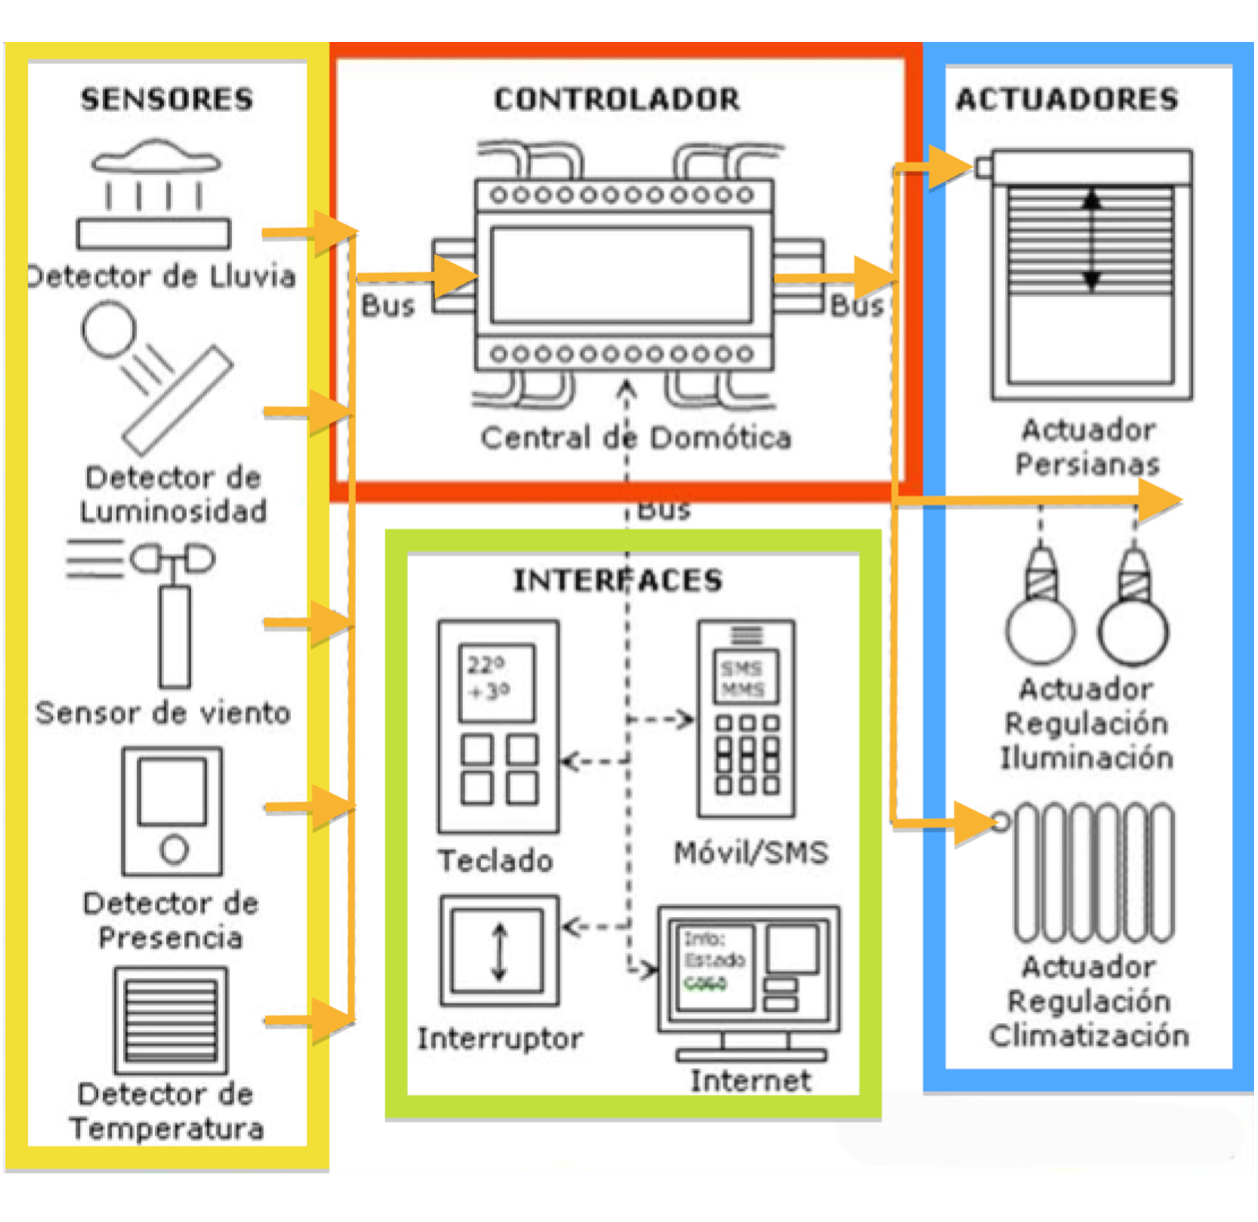
\includegraphics[width=.55\textwidth]{./Figures/domoticagenerico.png}
	\caption{Sistema de domótica genérico.}
	\label{fig:domoticagenerico}
\end{figure}

%--------------------------------------------------------------------------------------------------------------------------------

%\section{Descripción del problema}

%--------------------------------------------------------------------------------------------------------------------------------

\section{Estado del arte}

En la actualidad existe una amplia variedad de sistemas ofrecidos por empresas multinacionales como Fibaro, iHaus, Sonoff, ABB o Schneider Electric, que se encuentran enmarcados dentro de los sistemas de automatización y control de edificios/casas.Estos sistemas fueron tenidos en cuenta para la toma de decisiones en lo referente al desarrollo del trabajo, y por ello se resumen algunas características de estos en la tabla [\ref{tab:sistemasdomotica}].

\begin{table}[h]
	\centering
	\caption[Comparación]{Comparación de equipos en el mercado}
	\begin{tabular}{l c c c}    
		\toprule
		\textbf{Marcas}  	& \textbf{Conectividad}   	&\textbf{Interfaz}  	&\textbf{Monitoreo y Configuración}  						\\
		\midrule
		iHaus				& \ Zigbee 					&\ Display				&\ Software propietario										\\	
		Fibaro				& \ Z-wave					&\ No aplica			&\ WebServer												\\
		Sonoff	 			& \ Wifi/RF 				&\ Display				&\ Software propietario										\\
		ABB		 			& \ KNX 					&\ Display				&\ WebServer												\\
		Schneider E.	 	& \ BACNet 					&\ No aplica			&\ Software propietario										\\
		\bottomrule
		\hline
	\end{tabular}
	\label{tab:sistemasdomotica}
\end{table}

Si bien estos dispositivos se pueden adaptar a edificios de cualquier tipo, uno de los problemas mas usuales en cuanto a las conexiones inalámbricas es el alcance,es decir, la distancia entre el dispositivo central y el nodo. Los dispositivos mas comunes como los de iHaus, Fibaro y Sonoff son efectivos en cuanto al alcance en ámbitos residenciales, es decir, no están preparados para grandes distancias y muros anchos debido a que pierden la conectividad.

Otro aspecto a tener en cuenta en este tipo de dispositivos es la interfaz de usuario. Los sistemas de domótica en la actualidad proponen una gran variedad de opciones para visualizar la información de los sensores y actuadores, pero algunas opciones no terminan siendo aptas para un sistema de gestión en un edificio público y además se debe agregar mas hardware para dicho requerimiento.

En la figura [\ref{fig:ihausesquema}] se puede ver un esquema del sistema de iHaus como representación general de un sistema de domótica comercial \ref{fig:ihausesquema}. Éste cuenta con una central y nodos que funcionan como sensores y actuadores.

\begin{figure}[h]
	\centering
	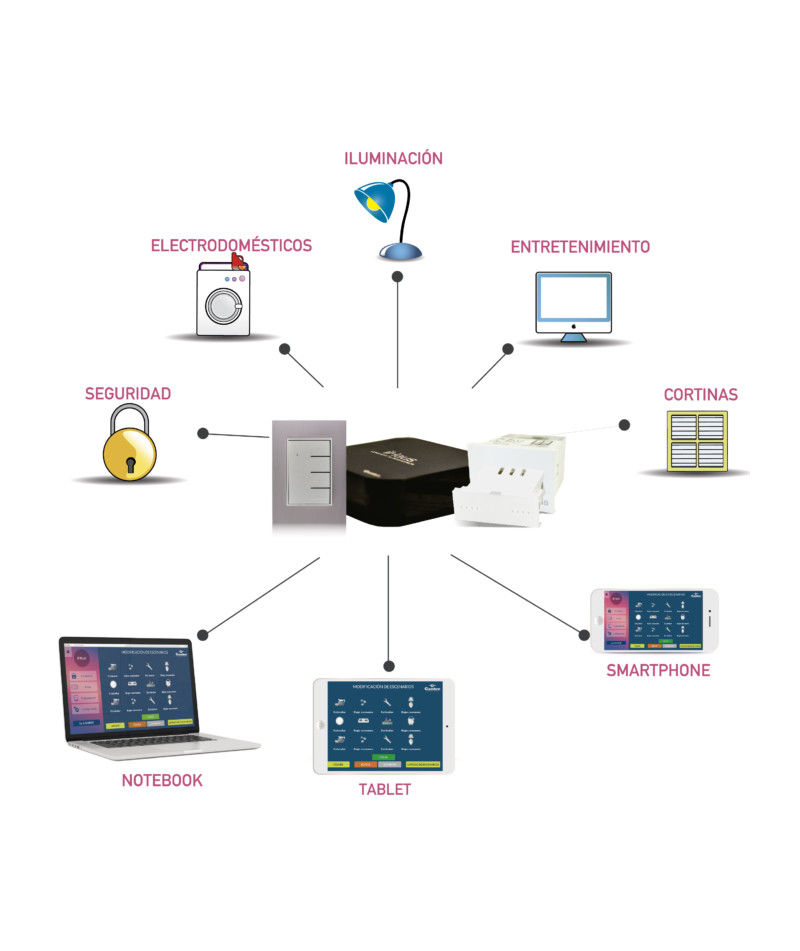
\includegraphics[width=.65\textwidth]{./Figures/ihausesquema.jpg}
	\caption{Sistema comercial de la marca iHaus.}
	\label{fig:ihausesquema}
\end{figure}

%--------------------------------------------------------------------------------------------------------------------------------

\section{Motivación}

%--------------------------------------------------------------------------------------------------------------------------------
Uno de los principales desafíos en la economía actual se refiere a la reducción en el uso de distintos tipos de energías (eléctrica, térmica, etc.) y la huella de CO\textsubscript{2} en los existentes edificios públicos utilizando tecnologías de la información, servicios de monitoreo y manejando el consumo de la energía. Se tiene especial atención a los edificios históricos que son generalmente menos eficientes energéticamente y requieren estrictas restricciones de despliegue para evitar daños por amplia actualización.
Un ámbito muy resignado por los desarrolladores de tecnología son los edificios públicos, debido a la complejidad en la instalación de este tipo de dispositivos. En la Argentina, en el marco del {\textit{Programa de Uso Racional y Eficiente de la Energía (PRONUREE) en Edificios Públicos}}, que tiene como objetivo reducir los niveles de consumo energético de la administración pública nacional mediante:

\begin{itemize}
\item La implementación de medidas de mejora de eficiencia energética.
\item La implementación de criterios para la gestión de la energía.
\item La concientización del personal en el uso racional de la energía.
\end{itemize}

Para cumplir con dicho marco se propone el desarrollo de un kit capaz de generar una red de sensores y actuadores que sean de fácil instalación y además que se pueda extender mediante el uso de la tecnología modular.
Disponer de estos dispositivos en edificios públicos tiene como beneficios:

\begin{itemize}
\item Monitoreo remoto de oficinas, aulas y espacios públicos.
\item Encendido y apagado de luces y aires acondicionados.
\item Mejora de la eficiencia energética de los edificios públicos.
\end{itemize}

En la figura [\ref{fig:esquemaplanteado}] se puede ver un esquema de la propuesta planteada.

\begin{figure}[h]
	\centering
	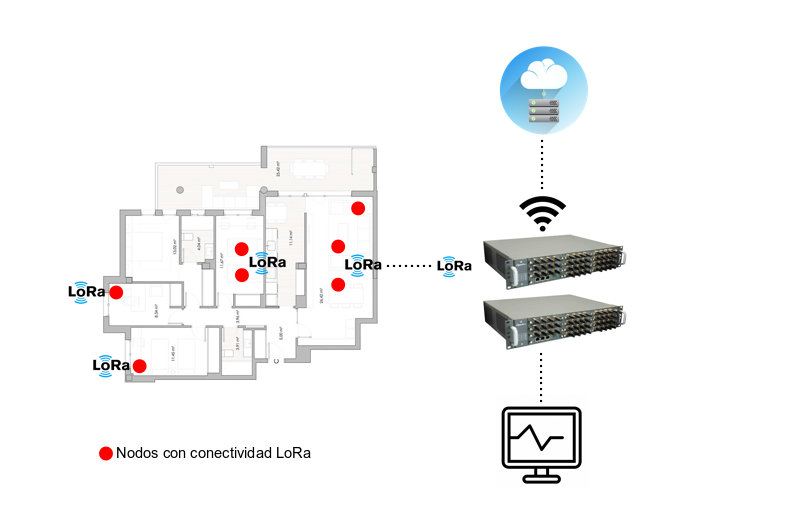
\includegraphics[width=.80\textwidth]{./Figures/esquemaplanteado.png}
	\caption{Esquema del sistema planteado.}
	\label{fig:esquemaplanteado}
\end{figure}


\section{Objetivos y alcances}
\label{sec:FillingFile}

En esta sección se hablará de los objetivos y alcances que tiene este proyecto.

\subsection{Objetivos}

El propósito de este proyecto es desarrollar un prototipo operativo de un sistema de control, monitoreo y supervisión de ciertas funciones y/o parámetros de los edificios, con la capacidad de visualizar la información de interés en un display e informar alertas. Un requisito importante es que su instalación requiera de una intervención mínima. Éste desarrollo permitirá maximizar la eficiencia del edificio, al reducir el consumo de energía y también generar alertas de prevención.

\subsection{Alcance}

Para la realización de este proyecto se desarrollará un primer prototipo operativo del sistema donde se tendrá en cuenta el hardware y software con interfaz de comunicación LoRa ({\textit{Long Range}}). El presente proyecto incluye los siguientes aspectos:

\begin{itemize}
\item Modelado del sistema.
\item Desarrollo del firmware de los nodos y el gateway.
\item Adquisición de datos de una serie de sensores en cada nodo de la red.
\item Transmisión de datos entre los nodos y el gateway mediante el uso del protocolo LoRa a 915 MHz.
\item Uso de base de datos en el gateway para guardar la información de cada nodo.
\item Visualización de los datos adquiridos y parámetros de configuración en una aplicación web.
\item Realización de tests y documentación detallados.
\end{itemize}

%--------------------------------------------------------------------------------------------------------------------------------

%\section{Bibliografía}
%\label{sec:biblio}
%
%Las opciones de formato de la bibliografía se controlan a través del paquete de latex \option{biblatex} que se incluye en la memoria en el archivo memoria.tex.  Estas opciones determinan cómo se generan las citas bibliográficas en el cuerpo del documento y cómo se genera la bibliografía al final de la memoria.
%
%En el preámbulo se puede encontrar el código que incluye el paquete biblatex, que no requiere ninguna modificación del usuario de la plantilla, y que contiene las siguientes opciones:
%
%\begin{lstlisting}
%\usepackage[backend=bibtex,
%	natbib=true, 
%	style=numeric, 
%	sorting=none]
%{biblatex}
%\end{lstlisting}
%
%En el archivo \file{reference.bib} se encuentran las referencias bibliográficas que se pueden citar en el documento.  Para incorporar una nueva cita al documento lo primero es agregarla en este archivo con todos los campos necesario.  Todas las entradas bibliográficas comienzan con $@$ y una palabra que define el formato de la entrada.  Para cada formato existen campos obligatorios que deben completarse. No importa el orden en que las entradas estén definidas en el archivo .bib.  Tampoco es importante el orden en que estén definidos los campos de una entrada bibliográfica. A continuación se muestran algunos ejemplos:
%
%\begin{lstlisting}
%@ARTICLE{ARTICLE:1,
%    AUTHOR="John Doe",
%    TITLE="Title",
%    JOURNAL="Journal",
%    YEAR="2017",
%}
%\end{lstlisting}
%
%
%\begin{lstlisting}
%@BOOK{BOOK:1,
%    AUTHOR="John Doe",
%    TITLE="The Book without Title",
%    PUBLISHER="Dummy Publisher",
%    YEAR="2100",
%}
%\end{lstlisting}
%
%
%\begin{lstlisting}
%@INBOOK{BOOK:2,
%    AUTHOR="John Doe",
%    TITLE="The Book without Title",
%    PUBLISHER="Dummy Publisher",
%    YEAR="2100",
%    PAGES="100-200",
%}
%\end{lstlisting}
%
%
%\begin{lstlisting}
%@MISC{WEBSITE:1,
%    HOWPUBLISHED = "\url{http://example.com}",
%    AUTHOR = "Intel",
%    TITLE = "Example Website",
%    MONTH = "12",
%    YEAR = "1988",
%    URLDATE = {2012-11-26}
%}
%\end{lstlisting}
%
%Se debe notar que los nombres \emph{ARTICLE:1}, \emph{BOOK:1}, \emph{BOOK:2} y \emph{WEBSITE:1} son nombres de fantasía que le sirve al autor del documento para identificar la entrada. En este sentido, se podrían reemplazar por cualquier otro nombre.  Tampoco es necesario poner : seguido de un número, en los ejemplos sólo se incluye como un posible estilo para identificar las entradas.
%
%La entradas se citan en el documento con el comando: 
%
%\begin{verbatim}
%\citep{nombre_de_la_entrada}
%\end{verbatim}
%
%Y cuando se usan, se muestran así: \citep{ARTICLE:1}, \citep{BOOK:1}, \citep{BOOK:2}, \citep{WEBSITE:1}.  Notar cómo se conforma la sección Bibliografía al final del documento. 

\chapter{Introducción específica} % Main chapter title

\label{Chapter2}

%----------------------------------------------------------------------------------------
%	SECTION 1
%----------------------------------------------------------------------------------------

En este capítulo se indican los requerimientos del sistema definidos junto con el cliente y posteriormente se realiza una breve introducción a las tecnologías utilizadas.

\section{Requerimientos}
\label{sec:introducción}

Durante el avance del proyecto surgieron cambios en los requerimientos, algunos sufrieron modificaciones muy pequeñas y se agregaron otros.
Las modificaciones en los requerimientos no generarían atrasos significativos con respecto al tiempo establecido para la finalización del proyecto.

\subsection{Requerimientos del nodo}

\begin{enumerate}
	\item 	Debe tener un relay (5v - 10A) para prender o apagar un dispositivo.
	\item 	Debe tener un módulo LoRa de 915MHz para comunicarse con el gateway.
	\item	Debe medir temperatura ambiente entre 0ºC y 40ºC con un resolución mínima de 8bits.
	\item	Debe tener una fuente switching de pequeño tamaño para suministrar energía a toda la placa del nodo.
	\item	La placa de circuito impreso deberá tener el tamaño tal que pueda ser utilizada en cajas de luz para embutir. Máximo 5x10cm.
	\item	Debe utilizar un led infrarrojo para enviar señales a los aires acondicionados.
	\item	Debe tener un pulsador para cambiar el modo de operación (manual o automático).
\end{enumerate}

\subsection{Requerimientos del gateway}

\begin{enumerate}
	\item	Debe tener un módulo LoRa de 915MHz para comunicarse con los nodos.
	\item	Debe tener conectividad Wi-Fi para comunicarse con el servidor.
	\item	Debe enviar la hora local a los nodos para sincronizar.
	\item	Debe enviar comandos a los nodos.
	\item	Debe tener conexión a un HMI.
\end{enumerate}

\subsection{Requerimientos del servidor}

\begin{enumerate}
	\item	Debe recibir información acerca de los nodos.
	\item	Debe ser accesible a través de una clave encriptada con Hash.
\end{enumerate}

En la figura [\ref{fig:requerimientos2}]se puede ver el sistema planteado para el proyecto con los periféricos mencionados en los requerimientos. En ésta se puede ver la separación entre el nodo y el gateway.

\begin{figure}[ht!]
	\centering
	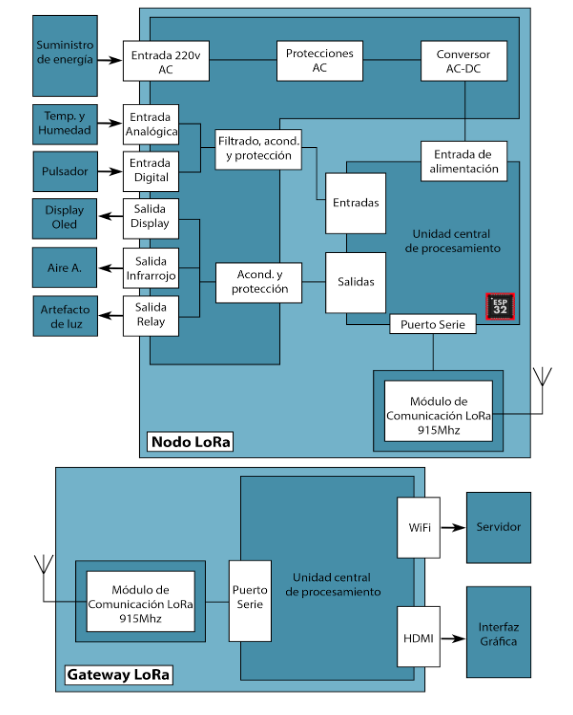
\includegraphics[width=1\textwidth]{./Figures/requerimientos2.png}
	\caption{Esquema general del sistema planteado.}
	\label{fig:requerimientos2}
\end{figure}

\section{Tecnología LoRa}
\label{sec:tecnologialora}

LoRa es un esquema patentado de modulación de espectro ensanchado que deriva de la modulación de espectro ensanchado Chirp (CSS). Establece una relación inversa entre velocidad de datos y sensibilidad dentro de un ancho de banda de canal fijo. Implementa una velocidad de datos variable, utilizando factores de ensanchamiento ortogonales que permiten al diseñador del sistema cambiar la velocidad de datos por rango o potencia, a fin de optimizar el rendimiento de la red en un ancho de banda constante.

LoRa es una implementación de capa física (PHY) y es independiente de las implementaciones de capa superior. Es utilizada en aplicaciones donde se requiere largo
alcance y bajo consumo con ancho de banda limitado, como se indica en la figura [\ref{fig:lora}].

\begin{figure}[ht!]
	\centering
	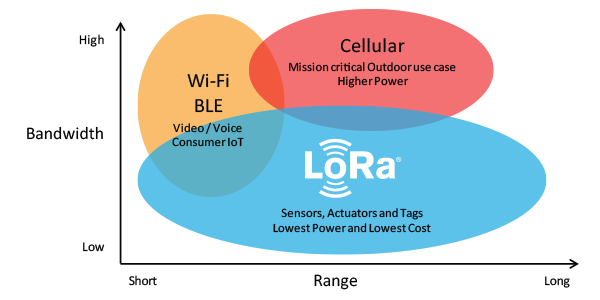
\includegraphics[width=0.8\textwidth]{./Figures/loragrafico.png}
	\caption{Campo de aplicación de tecnología de modulación LoRa.}
	\label{fig:lora}
\end{figure}

A continuación se introducen conceptos y se detallan brevemente las ventajas de la utilización de la tecnología LoRa.

El presupuesto de enlace (link budget) de un sistema o red inalámbrica es una medida de todas las ganancias y pérdidas desde el transmisor, a través del canal de propagación, hasta el receptor objetivo. Estas ganancias y pérdidas incluyen las ganancias y pérdidas del sistema asociadas con la antena, las redes coincidentes, etc., así como las pérdidas del canal de propagación asociado (ya sea a través de datos modelados o medidos).

Se dice que un canal de comunicaciones está limitado por el enlace cuando las pérdidas asociadas con el canal hacen que el nivel de potencia incidente en el receptor sea inferior al requerido para cumplir con el requisito de relación señal ruido (SNR) del receptor para la demodulación correcta de los datos recibidos.

La modulación LoRa es escalable en ancho de banda y frecuencia. Se puede utilizar tanto para salto de frecuencia de banda estrecha como para aplicaciones de secuencia directa de banda ancha. A diferencia de los esquemas de modulación de banda estrecha y banda ancha existentes, LoRa se puede adaptar fácilmente para cualquier modo de operación con solo modificar los registros de configuración del dispositivo.

Al igual que en la modulación por desplazamiento de frecuencia (FSK), LoRa es un esquema de modulación de envolvente constante, lo que significa que las mismas etapas amplificadoras de potencia (PA) de bajo costo y bajo consumo de energía pueden reutilizarse sin modificación. Además, debido a la ganancia de alcance asociada con LoRa, la potencia de salida del transmisor puede reducirse en comparación con un enlace FSK convencional.

Debido a su naturaleza asíncrona, una señal LoRa es muy resistente a los mecanismos de interferencia dentro y fuera de banda. Dado que el período del símbolo LoRa  puede ser más largo que la ráfaga típica de corta duración de los sistemas FHSS de salto rápido, proporciona una excelente inmunidad a los mecanismos de interferencia de AM pulsada. Para una potencia de salida y tasa de transferencia fijas, el presupuesto de enlace de LoRa excede el de FSK. Cuando se toma junto con la robustez probada ante interferencia y desvanecimiento de señal, esta mejora en el presupuesto de enlace puede traducirse fácilmente en un aumento del rango de alcance de más de cuatro veces.

La modulación LoRa emplea factores de ensanchamiento/dispersión ortogonales, lo que permite transmitir múltiples señales de propagación al mismo tiempo y en el mismo canal sin degradación de la sensibilidad de recepción. Las señales moduladas con diferentes factores de dispersión son percibidas como ruido por el receptor y son descartadas.

\section{Planificación}

En la figura [\ref{fig:activityonnode}] se puede ver el Diagrama de {\textit{activity-on-node}} que se presentó en el documento de planificación del proyecto.

\begin{figure}[ht!]
	\centering
	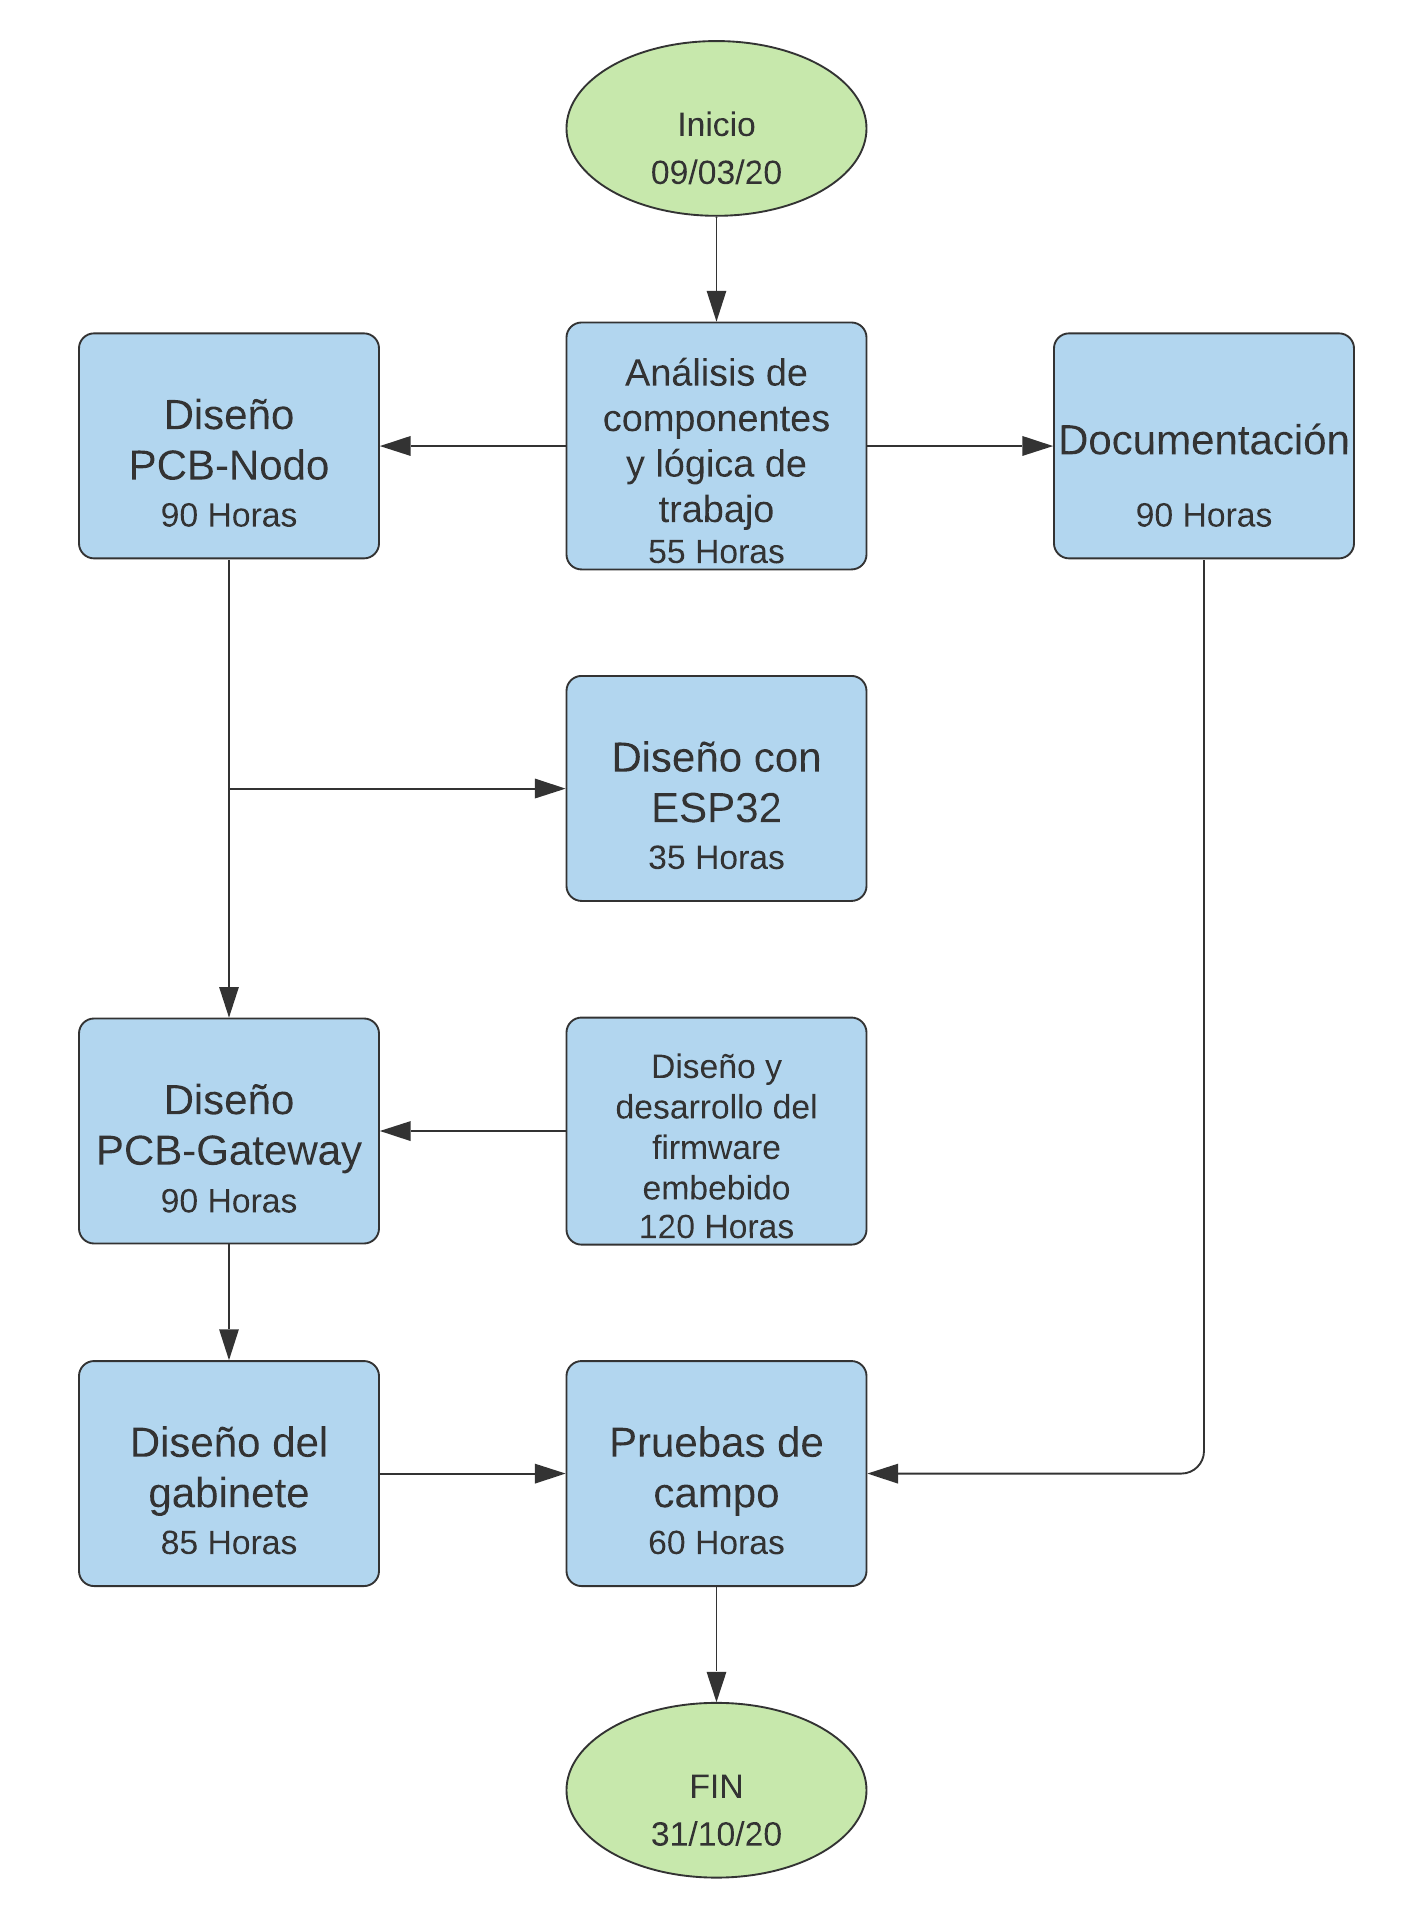
\includegraphics[width=0.8\textwidth]{./Figures/activityonnode.png}
	\caption{Diagrama de {\textit{activity-on-node.}}}
	\label{fig:activityonnode}
\end{figure}

Aquí se pueden ver las tareas a realizar y las horas que se lleva en cada una de las tareas. Cabe resaltar que las horas de la tarea "Diseño del PCB-Gateway" fueron destinadas finalmente al desarrollo del software y firmware del gateway.

 
\chapter{Diseño e implementación} % Main chapter title

\label{Chapter3} % Change X to a consecutive number; for referencing this chapter elsewhere, use \ref{ChapterX}

\definecolor{mygreen}{rgb}{0,0.6,0}
\definecolor{mygray}{rgb}{0.5,0.5,0.5}
\definecolor{mymauve}{rgb}{0.58,0,0.82}

%%%%%%%%%%%%%%%%%%%%%%%%%%%%%%%%%%%%%%%%%%%%%%%%%%%%%%%%%%%%%%%%%%%%%%%%%%%%%
% parámetros para configurar el formato del código en los entornos lstlisting
%%%%%%%%%%%%%%%%%%%%%%%%%%%%%%%%%%%%%%%%%%%%%%%%%%%%%%%%%%%%%%%%%%%%%%%%%%%%%
\lstset{ %
  backgroundcolor=\color{white},   % choose the background color; you must add \usepackage{color} or \usepackage{xcolor}
  basicstyle=\footnotesize,        % the size of the fonts that are used for the code
  breakatwhitespace=false,         % sets if automatic breaks should only happen at whitespace
  breaklines=true,                 % sets automatic line breaking
  captionpos=b,                    % sets the caption-position to bottom
  commentstyle=\color{mygreen},    % comment style
  deletekeywords={...},            % if you want to delete keywords from the given language
  %escapeinside={\%*}{*)},          % if you want to add LaTeX within your code
  %extendedchars=true,              % lets you use non-ASCII characters; for 8-bits encodings only, does not work with UTF-8
  %frame=single,	                % adds a frame around the code
  keepspaces=true,                 % keeps spaces in text, useful for keeping indentation of code (possibly needs columns=flexible)
  keywordstyle=\color{blue},       % keyword style
  language=[ANSI]C,                % the language of the code
  %otherkeywords={*,...},           % if you want to add more keywords to the set
  numbers=left,                    % where to put the line-numbers; possible values are (none, left, right)
  numbersep=5pt,                   % how far the line-numbers are from the code
  numberstyle=\tiny\color{mygray}, % the style that is used for the line-numbers
  rulecolor=\color{black},         % if not set, the frame-color may be changed on line-breaks within not-black text (e.g. comments (green here))
  showspaces=false,                % show spaces everywhere adding particular underscores; it overrides 'showstringspaces'
  showstringspaces=false,          % underline spaces within strings only
  showtabs=false,                  % show tabs within strings adding particular underscores
  stepnumber=1,                    % the step between two line-numbers. If it's 1, each line will be numbered
  stringstyle=\color{mymauve},     % string literal style
  tabsize=2,	                   % sets default tabsize to 2 spaces
  title=\lstname,                  % show the filename of files included with \lstinputlisting; also try caption instead of title
  morecomment=[s]{/*}{*/}
}

En éste capítulo se describe la estructura de la solución adoptada y el funcionamiento del hardware, software y firmware desarrollado específicamente para el cumplimiento de los requerimientos del sistema.

\section{Solución adoptada}

En base a los requerimientos enumerados en el capítulo 2, se desarrolló un sistema utilizando las tecnologías indicadas en la tabla [\ref{tab:solucionadoptada}].

\begin{table}[h]
	\centering
	\caption[Solución adoptada]{Tecnologías utilizadas en el desarrollo del sistema}
	\begin{tabular}{l m{4.5cm} m{4.5cm}}    
		\toprule
		\textbf{}  					& \textbf{Nodo}     				& \textbf{Gateway}	\\
		\midrule
		Aplicación 					& \ Firmware en C/C++				& \ Firmware en C/C++ y software en Python. \\
		Sistema operativo	 		& \ No corresponde 					& \ Linux\\
		Hardware		 			& \ ESP32(Xtensa LX6) 				& \ Raspberry pi 3(Cortex-A53) y ESP32(Xtensa LX6)\\
		\bottomrule
		\hline
	\end{tabular}
	\label{tab:solucionadoptada}
\end{table}

Se implementó el hardware del nodo en una placa de circuito impreso de diseño específico, descrito en la sección \ref{sec:nodos}. Contiene un microcontrolador de arquitectura MIPS({\textit{Microprocessor without Interlocked Pipeline Stages}}) de 32 bits. Cada nodo posee un circuito integrado de comunicación LoRa con su respectiva antena, sensores y actuadores, ésta permanece a la espera de recepción de comandos, conforme al protocolo propietario desarrollado.

Además se utilizó una raspberry pi como gateway descrito en la seccion \ref{sec:gateway}, a la cual se le conecta un hardware similar al nodo para utilizarlo como transceptor LoRa. La raspberry corre el sistema operativo Linux en la tarjeta microSD. También se desarrolló una aplicación en Python como {\textit{Backend}} de la interfaz web creada en {\textit{Node-red}}.


%----------------------------------------------------------------------------------------
%	SECTION 1
%----------------------------------------------------------------------------------------
\section{Arquitectura de funcionamiento}

En ésta sección se explica la arquitectura utilizada para la comunicación inalámbrica del sistema.
Se toma como referencia la arquitectura distribuida descrita en la sección \ref{sec:arquitecturadedomotica}. Ésta indica que la toma de decisiones por parte del sistema se encuentra en todos los dispositivos, no solo en uno central.
En la figura [\ref{fig:diagramadesecuencia}] se muestra el diagrama de secuencia del sistema. Éste se encuentra montado sobre una red inalámbrica local que utiliza el protocolo LoRa entre gateway y los nodos.

\begin{figure}[ht!]
	\centering
	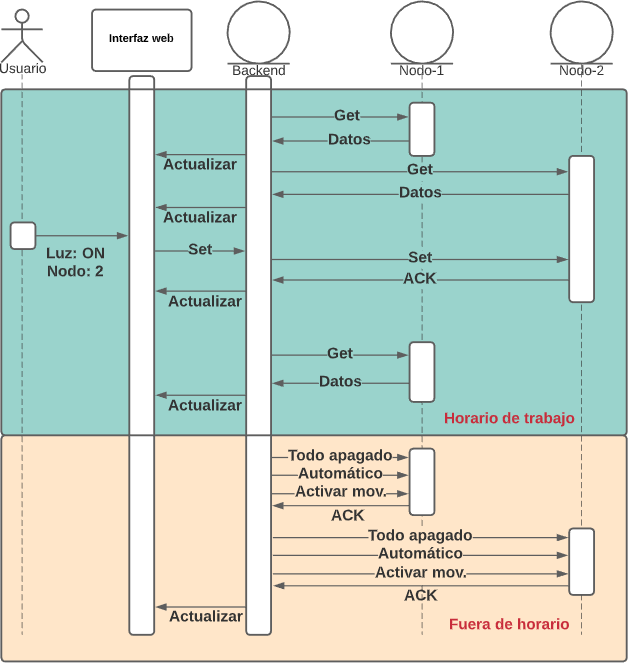
\includegraphics[width=0.8\textwidth]{./Figures/diagramadesecuencia.png}
	\caption{Diagrama de secuencia del sistema.}
	\label{fig:diagramadesecuencia}
\end{figure}

La arquitectura utilizada posee dos acciones posibles, estas son {\textit{Set}} y {\textit{Get}}. El objetivo de esta arquitectura es la de poder recibir datos con el comando {\textit{Get}} y configurar parámetros con el comando {\textit{Set}}, de ésta manera el sistema se reduce a una arquitectura simple y elemental que no genera grandes complicaciones en la programación de los dispositivos.
En este sistema, cuando existe un nodo o una red de nodos, el gateway se encuentra enviando el comando {\textit{Get}} a cada nodo en intervalos de 20 segundos. Ésto permite que la interfaz web se actualice constantemente. Al no ser un sistema crítico no se necesitan tiempos de respuesta rápidos por lo que 20 segundos es un tiempo prudente.
El nodo tiene permitido enviar datos sin antes haber recibido el comando {\textit{Get}}, solo cuando está en modo automático y tiene activado el sensor de movimiento.


%La idea de esta sección es resaltar los problemas encontrados, los criterios utilizados y la justificación de las decisiones que se hayan tomado.
%
%Se puede agregar código o pseudocódigo dentro de un entorno lstlisting con el siguiente código:
%
%\begin{verbatim}
%\begin{lstlisting}[caption= "un epígrafe descriptivo"]
%	las líneas de código irían aquí...
%\end{lstlisting}
%\end{verbatim}
%
%A modo de ejemplo:
%
%\begin{lstlisting}[label=cod:vControl,caption=Pseudocódigo del lazo principal de control.]  % Start your code-block
%
%#define MAX_SENSOR_NUMBER 3
%#define MAX_ALARM_NUMBER  6
%#define MAX_ACTUATOR_NUMBER 6
%
%uint32_t sensorValue[MAX_SENSOR_NUMBER];		
%FunctionalState alarmControl[MAX_ALARM_NUMBER];	//ENABLE or DISABLE
%state_t alarmState[MAX_ALARM_NUMBER];						//ON or OFF
%state_t actuatorState[MAX_ACTUATOR_NUMBER];			//ON or OFF
%
%void vControl() {
%
%	initGlobalVariables();
%	
%	period = 500 ms;
%		
%	while(1) {
%
%		ticks = xTaskGetTickCount();
%		
%		updateSensors();
%		
%		updateAlarms();
%		
%		controlActuators();
%		
%		vTaskDelayUntil(&ticks, period);
%	}
%}
%\end{lstlisting}

\section{Nodos}
\label{sec:nodos}

El nodo es el dispositivo del sistema del cual se extrae la información de los sensores y se utilizan sus actuadores para generar cambios en dispositivos externos al sistema inalámbrico como ser un aire acondicionado. En esta sección se explicara el hardware y parte del firmware del nodo.

\subsection{Hardware}

El hardware del nodo contiene los siguientes componentes:

\begin{enumerate}
\item Una fuente AC-DC de 220v a 5v. Figura [\ref{fig:esquematico1}].
\item Sensor de temperatura y humedad. Figura [\ref{fig:esquematico2}].
\item Modulo Heltec LoRa v2 con antena adaptada a 915MHz. Figura [\ref{fig:esquematico3}].
\item Circuito de leds infrarrojos. Figura [\ref{fig:esquematico4}].
\item Circuito relay. Figura [\ref{fig:esquematico5}].
\item Circuito de pulsadores. Figura [\ref{fig:esquematico6}].
\item Circuito de leds indiciadores. Figura [\ref{fig:esquematico7}].
\end{enumerate}

En la figura [\ref{fig:esquematico1}] se tiene el circuito de la fuente. Se decidió buscar en el mercado una fuente compacta y pequeña debido al tamaño final que debe tener el producto. Se utilizó la fuente compacta HLK-PM01 de la empresa Hi-Link.

\begin{figure}[h!]
	\centering
	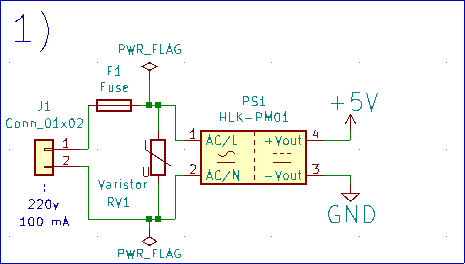
\includegraphics[width=0.6\textwidth]{./Figures/esquematico1.png}
	\caption{Circuito de fuente AC-DC.}
	\label{fig:esquematico1}
\end{figure}

En la figura [\ref{fig:esquematico2}] se muestra el circuito del sensor de temperatura y humedad. El sensor es el conocido DHT11 que tiene un rango de temperatura de 0 a 50 ºC con 5\% de precisión y un rango de humedad de 20 al 80 \% con una precisión del 5\%.

\begin{figure}[h!]
	\centering
	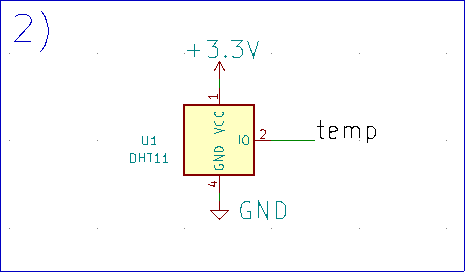
\includegraphics[width=0.6\textwidth]{./Figures/esquematico2.png}
	\caption{Circuito de sensor de temperatura.}
	\label{fig:esquematico2}
\end{figure}

En la figura [\ref{fig:esquematico3}] se ve el circuito de conectores que ofician de zócalo para conectar el modulo externo Heltec LoRa v2. Éste módulo fue elegido debido a que ofrece un microcontrolador esp32 de arquitectura Tensilica Xtensa LX6 de 32bits por lo que se utiliza como controlador principal del nodo, además posee un display oled y el circuito integrado {\textit{SX1276}} de la empresa Semtech, con conector Hirose U.FL para antenas miniatura de RF de hasta 6 GHz.

\begin{figure}[h!]
	\centering
	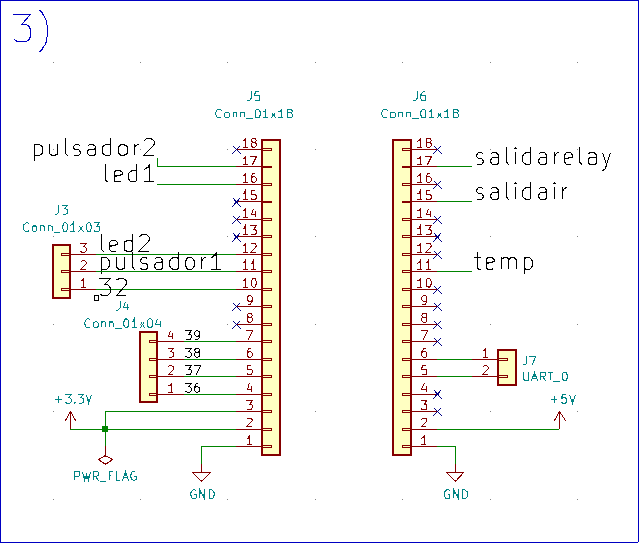
\includegraphics[width=0.6\textwidth]{./Figures/esquematico3.png}
	\caption{Conectores para el modulo Heltec LoRa v2.}
	\label{fig:esquematico3}
\end{figure}

En la figura [\ref{fig:esquematico4}] se ve un circuito típico para el uso de leds en general. Se utilizaron dos leds debido a que en las pruebas se obtuvo mayor alcance del haz infrarrojo con respecto a los aires acondicionados. El led infrarrojo es el actuador para el encendido y apagado de los aires acondicionados.

\begin{figure}[h!]
	\centering
	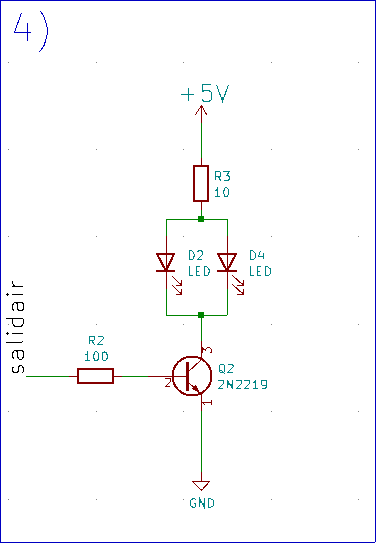
\includegraphics[width=0.4\textwidth]{./Figures/esquematico4.png}
	\caption{Circuito de leds infrarrojos.}
	\label{fig:esquematico4}
\end{figure}

En la figura [\ref{fig:esquematico5}] se tiene un circuito típico de relay con su respectivo conector de salida. El relay es el actuador para el encendido y apagado de la luz.

\begin{figure}[h!]
	\centering
	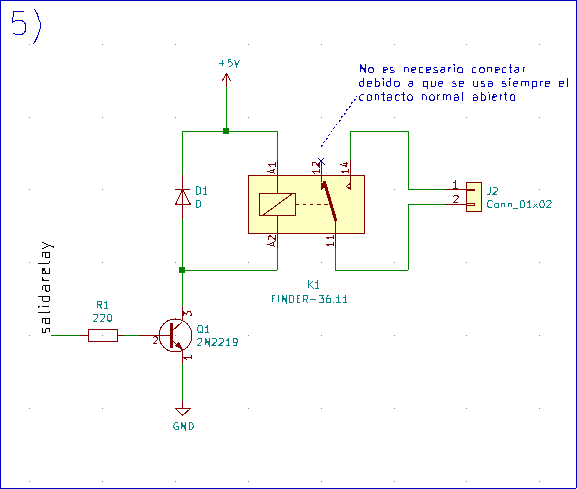
\includegraphics[width=0.6\textwidth]{./Figures/esquematico5.png}
	\caption{Circuito de relay.}
	\label{fig:esquematico5}
\end{figure}

En la figura [\ref{fig:esquematico6}] se muestra el circuito de los pulsadores, éstos son el pulsador de {\textit{Modo}} que se utiliza para sincronizar el nodo con el gateway y además para cambiar el modo de manual a automático, y el pulsador para encendido y apagado de la luz.

\begin{figure}[h!]
	\centering
	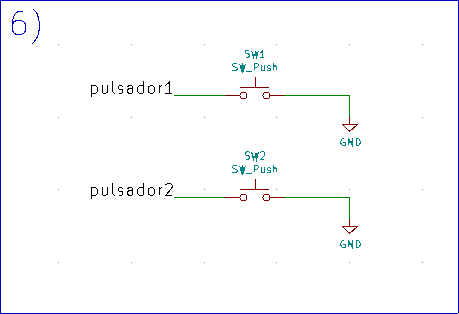
\includegraphics[width=0.5\textwidth]{./Figures/esquematico6.png}
	\caption{Circuito de pulsadores.}
	\label{fig:esquematico6}
\end{figure}

En la figura [\ref{fig:esquematico7}] se muestra el circuito de leds indicadores, se utilizan para debugging del sistema.

\begin{figure}[h!]
	\centering
	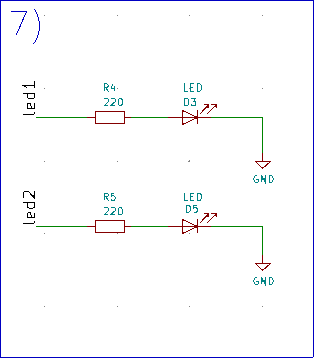
\includegraphics[width=0.4\textwidth]{./Figures/esquematico7.png}
	\caption{Circuito de leds indicadores.}
	\label{fig:esquematico7}
\end{figure}

La imagen renderizada de la placa de circuito impreso desarrollada en la herramienta libre Kicad, se muestra en la figura [\ref{fig:pcb1}].

\begin{figure}[h!]
	\centering
	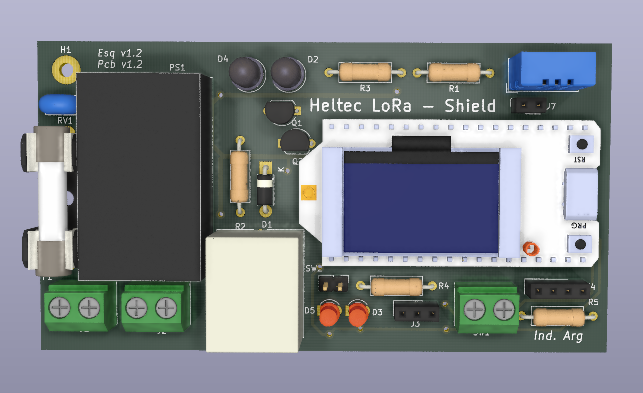
\includegraphics[width=0.6\textwidth]{./Figures/pcb1.png}
	\caption{Render de placa de circuito impreso.}
	\label{fig:pcb1}
\end{figure} 

En la figura [\ref{fig:pcb2}] se puede ver la imagen de la pcb realizada. Ésta es una pcb de doble capa, realizada de forma casera con el método de insolación ultravioleta.

\begin{figure}[h!]
	\centering
	\includegraphics[width=0.6\textwidth]{./Figures/pcb2.png}
	\caption{Placa de circuito impreso.}
	\label{fig:pcb2}
\end{figure} 

\subsection{Firmware}

La arquitectura del firmware se diseño teniendo en cuenta algunos patrones de diseño de arquitectura y conceptos de programación orientada a objetos en C/C++.
Para el desarrollo del firmware se utilizó la API que provee el fabricante del módulo Heltec LoRa, éste provee los drivers de la siguiente lista:

\begin{itemize}
\item Display Oled 128x64.
\item Protocolo LoRa.
\end{itemize}

Además se utilizó una librería creada para el uso de infrarrojos con el microcontrolador ESP32, con el objetivo de agilizar el desarrollo ya que existe una gran variedad de aires acondicionados y protocolos muy variados. Se encontró que la librería provee 92 protocolos, es decir, 92 dispositivos distintos a los cuales se los puede manipular con infrarrojo. Si bien la API de la empresa {\textit{Espressif}}(ESP-IDF), está desarrollada completamente sobre el sistema operativo de tiempo real freeRTOS. Se utilizó como API principal la de Arduino debido a que el sistema no necesita ser de tiempo real, ésta provee soluciones que agilizan el desarrollo de este tipo de dispositivos.

El firmware posee un arquitectura en capas, esto permite la separación de las partes que componen el sistema. En la figura [\ref{fig:capas}] se pueden ver las capas que componen el sistema.

\begin{figure}[h!]
	\centering
	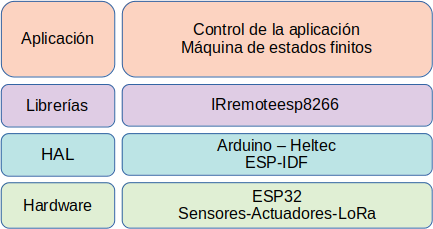
\includegraphics[width=0.6\textwidth]{./Figures/capas.png}
	\caption{Arquitectura en capas del firmware del nodo.}
	\label{fig:capas}
\end{figure}












\section{Gateway}
\label{sec:gateway}

blablaba

\section{Interfaz web}

blabla

\section{Backend del sistema}

blabla


% Chapter Template

\chapter{Ensayos y Resultados} % Main chapter title

\label{Chapter4} % Change X to a consecutive number; for referencing this chapter elsewhere, use \ref{ChapterX}

En este capítulo se detallan los ensayos realizados para comprobar el correcto funcionamiento del firmware de los nodos y el {\textit{Gateway}}, como así también del sistema en general.
%----------------------------------------------------------------------------------------
%	SECTION 1
%----------------------------------------------------------------------------------------

\section{Ensayos de comunicación}
\label{sec:pruebasHW}

En esta sección se detallan los ensayos de comunicación entre el nodo y el {\textit{gateway}} a partir de una terminal de comandos en Linux. Estos ensayos son muy importantes debido a que la comunicación inalámbrica es el requerimiento principal del proyecto. El objetivo es comprobar que existe una correcta comunicación entre los dos dispositivos.

\subsection{Banco de pruebas}

El banco de pruebas de ésta sección se componen de los elementos listados en la tabla [\ref{tab:bancodepruebas1}] :

\begin{table}[h]
	\centering
	\caption[Banco de pruebas 1]{Banco de pruebas para ensayos de comunicación}
	\begin{tabular}{l c m{7.5cm}}    
		\toprule
		\textbf{Componentes}  		& \textbf{Pertenencia}     	& \textbf{Función}																				\\
		\midrule
		Raspberry Pi				& \ Gateway 				& \ Funciona como nexo entre entre el transceptor y una terminal para enviar comandos por UART.	\\
		Transceptor LoRa 			& \ Gateway					& \ Conectado a través de la UART, recibe comandos y los envía por LoRa (915 MHz). 				\\
		Display	 					& \ Gateway 				& \ Conectado al puerto HDMI de la raspberry pi. 												\\
		Transceptor LoRa		 	& \ Nodo 					& \ Recibe comandos por LoRa, los procesa, ejecuta y envía una respuesta.						\\
		\bottomrule
		\hline
	\end{tabular}
	\label{tab:bancodepruebas1}
\end{table}

La propuesta de éste banco es la de tener los componentes mínimos y necesarios al hacer las pruebas de conectividad y de {\textit{Set/Get}} mediante una terminal de comandos. En la figura [\ref{fig:bancodepruebas1}] se puede ver el esquema de conexión básico.

\begin{figure}[ht!]
	\centering
	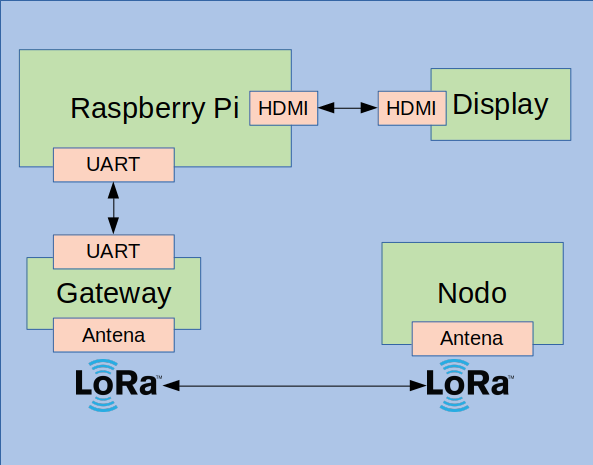
\includegraphics[width=0.5\textwidth]{./Figures/bancodepruebas.png}
	\caption{Banco de pruebas para el ensayo de comunicación.}
	\label{fig:bancodepruebas1}
\end{figure}

\subsection{Pruebas}

\subsubsection{Pruebas de conexión}
El nodo posee dos estados de conectividad inalámbrica, éstos estados son conectado y desconectado. En ésta prueba se logra realizar la conexión inalámbrica de un nodo con el {\textit{gateway}}. Los pasos realizados fueron los siguientes:

\begin{enumerate}
\item Con el nodo encendido, presionar el botón {\textit{Modo}} por seis segundos.
\end{enumerate}

En la figura [\ref{fig:conexion}] se puede ver que el {\textit{gateway}} recibe el comando NODE:ID, donde ID corresponde al nodo utilizado. Cuando el {\textit{gateway}} recibe éste comando, envía un {\textit{ACK}} al nodo y éste pasa al estado conectado.

\begin{figure}[h!]
	\centering
	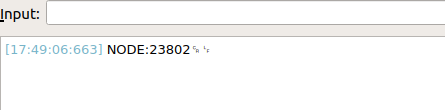
\includegraphics[width=0.5\textwidth]{./Figures/conexion.png}
	\caption{Ensayo de conexión de un nuevo nodo.}
	\label{fig:conexion}
\end{figure}

\subsubsection{Pruebas de Set y Get}
Las pruebas realizadas en esta sección corresponden al envío de comandos para configurar o setear algún parámetro del nodo y también recibir información de éste.
Los pasos realizados fueron los siguientes:

\begin{enumerate}
\item Enviar el comando {\textit{Get}} y esperar a recibir un array de datos.
\item Enviar el comando correspondiente para configurar el estado del sistema al modo {\textit{Manual}} y esperar un {\textit{ACK}}.
\item Enviar nuevamente el comando {\textit{Get}} para corroborar el seteo del parámetro.
\end{enumerate}

En la figura [\ref{fig:image1}] se puede ver el paso 1, donde en la figura [\ref{fig:get1}] se envía el comando y en la figura [\ref{fig:get2}] se recibe el {\textit{ACK}}.

\begin{figure}[h]

\begin{subfigure}{0.5\textwidth}
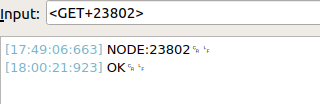
\includegraphics[width=1\textwidth]{./Figures/GET1.png}
\caption{Envío del comando {\textit{Get}} por consola al puerto serie.}
\label{fig:get1}
\end{subfigure}
\begin{subfigure}{0.5\textwidth}
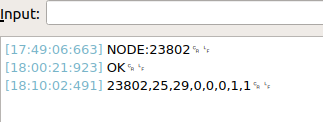
\includegraphics[width=1\textwidth]{./Figures/GET2.png}
\caption{Recepción de datos enviados por el nodo.}
\label{fig:get2}
\end{subfigure}

\caption{}
\label{fig:image1}
\end{figure}

En la figura [\ref{fig:image2}] se puede ver el paso 2, donde en la figura [\ref{fig:confmanual1}] se envía el comando y en la [\ref{fig:confmanual2}] se recibe el {\textit{ACK}}.

\begin{figure}[h]

\begin{subfigure}{0.5\textwidth}
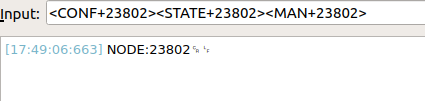
\includegraphics[width=1\textwidth]{./Figures/CONFMANUAL1.png}
\caption{Envío del comando {\textit{Conf}} para poner el sistema en modo manual.}
\label{fig:confmanual1}
\end{subfigure}
\begin{subfigure}{0.5\textwidth}
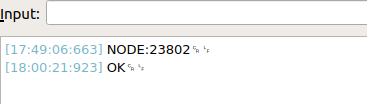
\includegraphics[width=1\textwidth]{./Figures/CONFMANUAL2.png}
\caption{Recepción del comando {\textit{Ok}} enviado por el nodo.}
\label{fig:confmanual2}
\end{subfigure}

\caption{}
\label{fig:image2}
\end{figure}

Finalmente en la figura [\ref{fig:confmanual3}] se puede ver la recepción del comando {\textit{Get}} que corresponde al paso 3 y se corrobora el cambio en el parámetro.

\begin{figure}[ht!]
	\centering
	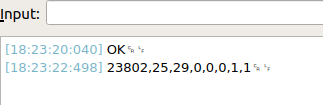
\includegraphics[width=0.5\textwidth]{./Figures/CONFMANUAL3.png}
	\caption{Recepción de datos enviados por el nodo.}
	\label{fig:confmanual3}
\end{figure}


\subsubsection{Resultados}

\begin{itemize}
\item Se comprobó que la arquitectura de comandos utilizada funciona correctamente.
\item El envío y recepción de datos toma un tiempo menor a 2 segundos por comando.
\item El nodo procesa satisfactoriamente la información.
\end{itemize}


\section{Ensayos de sensores y actuadores}

En esta sección se detallan los ensayos de uso de los periféricos en el nodo, comandados por el {\textit{gateway}}. El objetivo de estos ensayos es corroborar el correcto funcionamiento de la placa de circuitos impreso desarrollada, como también los sensores y actuadores utilizados.

\subsection{Banco de pruebas}

El banco de pruebas de ésta sección se componen de los elementos listados en la tabla [\ref{tab:bancodepruebas2}]:

\begin{table}[h]
	\centering
	\caption[Banco de pruebas 1]{Banco de pruebas para ensayos de comunicación}
	\begin{tabular}{l c m{7.5cm}}    
		\toprule
		\textbf{Componentes}  		& \textbf{Pertenencia}     	& \textbf{Función}																				\\
		\midrule
		Raspberry Pi				& \ Gateway 				& \ Funciona como nexo entre entre el transceptor y una terminal para enviar comandos por UART.	\\
		Transceptor LoRa 			& \ Gateway					& \ Conectado a través de la UART, recibe comandos y los envía por LoRa (915 MHz). 				\\
		Display	 					& \ Gateway 				& \ Conectado al puerto HDMI de la raspberry pi. 												\\
		Transceptor LoRa		 	& \ Nodo 					& \ Recibe comandos por LoRa, los procesa, ejecuta y envía una respuesta.						\\
		Periféricos		 			& \ Nodo 					& \ Sensor de movimiento, sensor de temperatura y humedad, relay y led infrarrojo				\\
		\bottomrule
		\hline
	\end{tabular}
	\label{tab:bancodepruebas2}
\end{table}

En la figura [\ref{fig:bancodepruebas2}] se puede ver el esquema de conexionado básico.

\begin{figure}[h!]
	\centering
	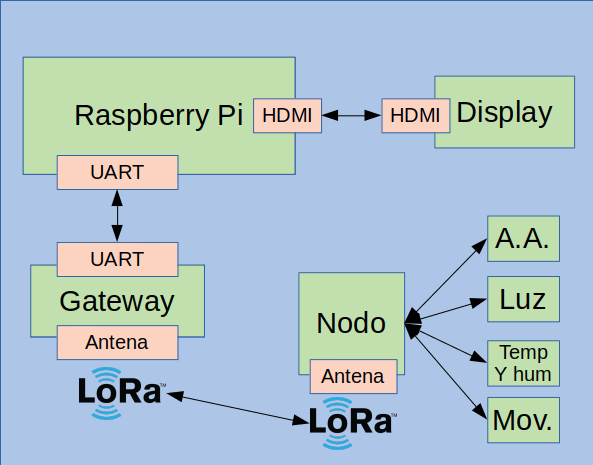
\includegraphics[width=0.5\textwidth]{./Figures/bancodepruebas1.png}
	\caption{Banco de pruebas para el ensayo de sensores y actuadores.}
	\label{fig:bancodepruebas2}
\end{figure}

\subsection{Pruebas}

Las pruebas realizadas fueron de encendido y apagado de luz y aire acondicionado, detección de movimiento y sensado de temperatura y humedad.

Se comprobó el correcto funcionamiento de forma visual en los dispositivos y además utilizando el comando {\textit{Get}} para determinar si hubo un cambio en el estado de las salidas.

\subsubsection{Pruebas de encendido y apagado de luces}

Los pasos realizados en éste ensayo fueron los siguientes:

\begin{enumerate}
\item Enviar el comando para encender la luz, esperar un {\textit{ACK}}.
\item Enviar el comando {\textit{Get}} y esperar un array de datos de respuesta.
\item Enviar el comando para apagar la luz, esperar un {\textit{ACK}}.
\item Enviar el comando {\textit{Get}} y esperar un array de datos de respuesta.
\end{enumerate}

En la figura [\ref{fig:image3}] se puede ver el paso 1 y 2, donde en la figura [\ref{fig:luz1}] se envía el comando y en la figura [\ref{fig:luz2}] se recibe el {\textit{ACK}} y el array de datos.

\begin{figure}[h]

\begin{subfigure}{0.5\textwidth}
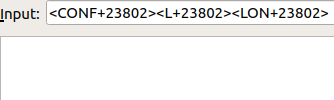
\includegraphics[width=1\textwidth]{./Figures/luz1.png}
\caption{Envío de comando para encender la luz.}
\label{fig:luz1}
\end{subfigure}
\begin{subfigure}{0.5\textwidth}
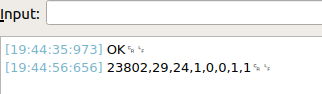
\includegraphics[width=1\textwidth]{./Figures/luz2.png}
\caption{Recepción de datos.}
\label{fig:luz2}
\end{subfigure}

\caption{}
\label{fig:image3}
\end{figure}

En la figura [\ref{fig:image4}] se puede ver el paso 3 y 4, donde en la figura [\ref{fig:luz3}] se envía el comando y en la figura [\ref{fig:luz4}] se recibe el {\textit{ACK}} y el array de datos.

\begin{figure}[h]

\begin{subfigure}{0.5\textwidth}
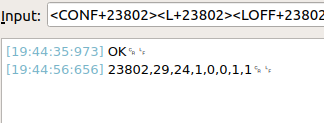
\includegraphics[width=1\textwidth]{./Figures/luz3.png}
\caption{Envío de comando para apagar la luz.}
\label{fig:luz3}
\end{subfigure}
\begin{subfigure}{0.5\textwidth}
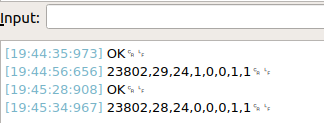
\includegraphics[width=1\textwidth]{./Figures/luz4.png}
\caption{Recepción de datos.}
\label{fig:luz4}
\end{subfigure}

\caption{}
\label{fig:image4}
\end{figure}

Si se comparan los dos arrays de datos en la figura [\ref{fig:luz4}] se puede ver claramente el cambio de la variable en la columna 4.

\subsubsection{Pruebas de encendido y apagado de aire acondicionado}

Los pasos realizados en éste ensayo fueron los siguientes:

\begin{enumerate}
\item Enviar cambio de protocolo de aire acondicionado y esperar un {\textit{ACK}}.
\item Enviar el comando para encender el aire acondicionado, esperar un {\textit{ACK}}.
\item Enviar el comando {\textit{Get}} y esperar un array de datos de respuesta.
\item Enviar el comando para apagar el aire acondicionado, esperar un {\textit{ACK}}.
\item Enviar el comando {\textit{Get}} y esperar un array de datos de respuesta.
\end{enumerate}

En la figura [\ref{fig:aa1}] se puede ver la secuencia de comandos recibidos por el {\textit{gateway}} correspondiente a la secuencia descrita anteriormente.

\begin{figure}[h!]
	\centering
	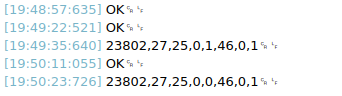
\includegraphics[width=0.55\textwidth]{./Figures/aa1.png}
	\caption{Respuestas del nodo a los comandos utilizados.}
	\label{fig:aa1}
\end{figure}

Si se comparan los dos arrays de datos en la figura [\ref{fig:aa1}] se puede ver claramente el cambio de la variable en la columna 5.

\subsubsection{Pruebas de sensores}

El sistema posee dos sensores, un sensor de humedad y temperatura y un sensor de movimiento. El objetivo de este ensayo es corroborar el correcto funcionamiento de estos. Los pasos para los ensayos del sensor de temperatura y humedad fueron los siguientes:

\begin{enumerate}
\item Enviar el comando {\textit{Get}} para conocer el valor de temperatura y humedad actual.
\item Acercar una fuente de calor al sensor.
\item Enviar el comando {\textit{Get}} para corroborar el cambio de temperatura y humedad.
\end{enumerate}

En la figura [\ref{fig:sensores1}] se puede ver la respuesta del sensor a los dos envíos del comando {\textit{Get}} y se puede corroborar que los valores de temperatura y humedad han cambiado. Estos valor se pueden ver en el array, en las columnas 2 (temperatura) y 3(humedad).

\begin{figure}[h!]
	\centering
	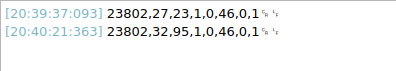
\includegraphics[width=0.55\textwidth]{./Figures/sensores1.png}
	\caption{Respuesta al cambio de temperatura y humedad en el nodo.}
	\label{fig:sensores1}
\end{figure}

Finalmente se hizo el ensayo del sensor de movimiento, para el que se siguieron los pasos:

\begin{enumerate}
\item Enviar el comando para cambiar el estado del sistema a {\textit{Automático}} y esperar un {\textit{ACK}}.
\item Enviar el comando para activar el sensor de movimiento y esperar un {\textit{ACK}}.
\item Mover un objeto frente al sensor de movimiento.
\end{enumerate}

En la figura [\ref{fig:sensores2}] se puede ver la secuencia descrita anteriormente. Se reciben los dos {\textit{ACK}} y luego se procede al paso 3 que genera el envío del comando de alarma del nodo al {\textit{gateway}}.

\begin{figure}[h!]
	\centering
	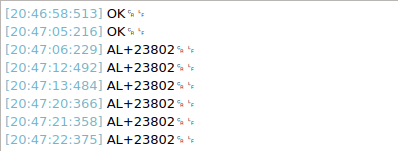
\includegraphics[width=0.55\textwidth]{./Figures/sensores2.png}
	\caption{Pruebas del sensor de movimiento.}
	\label{fig:sensores2}
\end{figure}

\subsubsection{Resultados}

\begin{itemize}
\item Se comprobó que los sensores y actuadores funcionan correctamente.
\item El envío de datos al sensar movimiento tiene un tiempo menor a 2 segundos y lo hace de forma correcta.
\item El circuito impreso desarrollado funciona correctamente.
\end{itemize}


\section{Ensayos de integración}

En esta sección se detallan los ensayos de comunicación entre el nodo y el {\textit{gateway}}, para ello se utiliza una interfaz web y un proceso programado en {\textit{Python}} que maneja las peticiones de la interfaz de usuario creada en {\textit{Node-red}}. El objetivo de estos ensayos es corroborar el correcto funcionamiento del sistema con el agregado de la interfaz web y simulando el sistema completo.

\subsection{Banco de pruebas}

El banco de pruebas de ésta sección se componen de los elementos listados en la tabla [\ref{tab:bancodepruebas3}]:

\begin{table}[h]
	\centering
	\caption[Banco de pruebas 1]{Banco de pruebas para ensayos de comunicación}
	\begin{tabular}{l c m{7.5cm}}    
		\toprule
		\textbf{Componentes}  		& \textbf{Pertenencia}     	& \textbf{Función}																				\\
		\midrule
		Raspberry Pi				& \ Gateway 				& \ Ejecuta la aplicación programada en {\textit{Python}} y la interfaz web.	\\
		Transceptor LoRa 			& \ Gateway					& \ Conectado a través de la UART, recibe comandos y los envía por LoRa (915 MHz). 				\\
		Display	 					& \ Gateway 				& \ Conectado al puerto HDMI de la raspberry pi. 												\\
		Transceptor LoRa		 	& \ Nodo 					& \ Recibe comandos por LoRa, los procesa, ejecuta y envía una respuesta.						\\
		Periféricos		 			& \ Nodo 					& \ Sensor de movimiento, sensor de temperatura y humedad, relay y led infrarrojo				\\
		\bottomrule
		\hline
	\end{tabular}
	\label{tab:bancodepruebas3}
\end{table}

En la figura [\ref{fig:bancodepruebas3}] se puede ver el esquemático básico del sistema. Se utiliza la ventana de comandos con el motivo de mostrar que los comandos son enviados correctamente cuando se interactúa con la interfaz web. 

\begin{figure}[ht!]
	\centering
	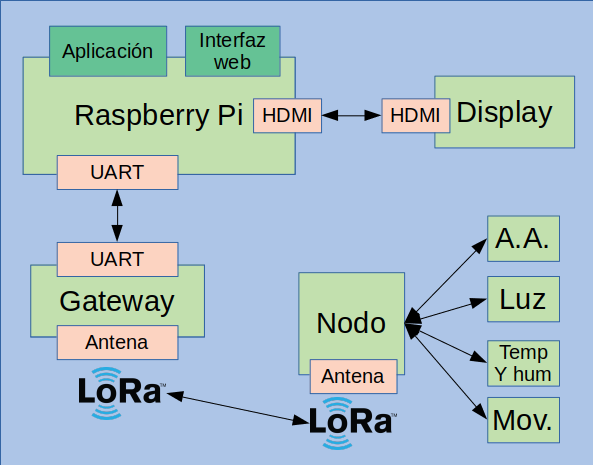
\includegraphics[width=0.5\textwidth]{./Figures/bancodepruebas2.png}
	\caption{Banco de prueba para ensayos de integración.}
	\label{fig:bancodepruebas3}
\end{figure}


\subsection{Pruebas}

Las pruebas realizadas se detallan en la siguiente lista:

\begin{enumerate}
\item Ensayo de conexión con interfaz y aplicación.
\item Ensayo de encendido y apagado de luz.
\item Ensayo de encendido y apagado de aire acondicionado.
\item Ensayo de sensor de temperatura y humedad.
\item Ensayo de sensor de movimiento.
\end{enumerate}

\subsubsection{Pruebas de conexión con interfaz y aplicación}

Se realizó el ensayo de conexión de un nodo al sistema mediante el uso de la interfaz web. Para ello se siguen los pasos:

\begin{enumerate}
\item Hacer click en la solapa {\textit{Configuración}}.
\item Hacer click en {\textit{Agregar nuevo dispositivo}}.
\item Presionar el botón {\textit{Modo}} del nodo durante seis segundos.
\end{enumerate}

En las figuras [\ref{fig:interfaz1}] y [\ref{fig:interfaz2}] se ven los pasos 1 y 2. Aquí se selecciona la solapa de configuración para tener disponible el botón de agregado de un nodo al sistema.

\begin{figure}[ht!]
	\centering
	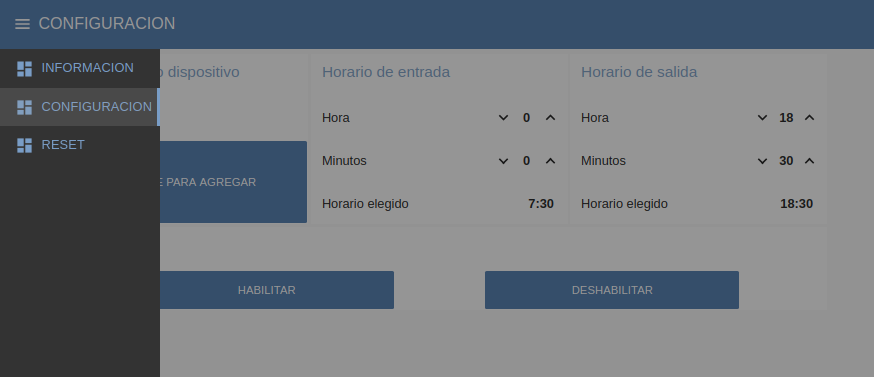
\includegraphics[width=0.8\textwidth]{./Figures/interfaz1.png}
	\caption{Solapa de configuración.}
	\label{fig:interfaz1}
\end{figure}

\begin{figure}[ht!]
	\centering
	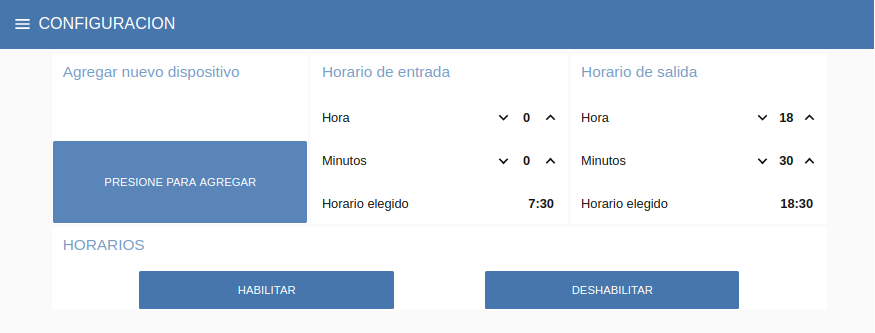
\includegraphics[width=0.8\textwidth]{./Figures/interfaz2.png}
	\caption{Ventana de configuración.}
	\label{fig:interfaz2}
\end{figure}

En la figura [\ref{fig:interfaz3}] se muestra la terminal de Linux en la que luego del paso 3 mencionado, llega el comando NODE:ID correspondiente al nodo en cuestión. Finalmente el sistema escribe en un archivo de log, la línea que se muestra en la parte inferior de la figura.

\begin{figure}[ht!]
	\centering
	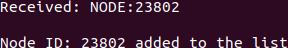
\includegraphics[width=0.5\textwidth]{./Figures/interfaz3.png}
	\caption{Terminal de comandos muestra recepción del nodo.}
	\label{fig:interfaz3}
\end{figure}

\subsubsection{Pruebas de encendido y apagado de luz}

Se realizó el ensayo de encendido y apagado de luz mediante el uso de los botones ON y OFF de la interfaz web, correspondientes al nodo en cuestión. Para ello se siguen los pasos:

\begin{enumerate}
\item Hacer click en la solapa {\textit{Información}}.
\item Hacer click en {\textit{ON}}.
\item Hacer click en {\textit{OFF}}.
\end{enumerate}

En la figura [\ref{fig:interfaz4}] se puede ver el paso 1, aquí se selecciona la solapa de información que se encuentra en la parte izquierda de la pagina web.

\begin{figure}[ht!]
	\centering
	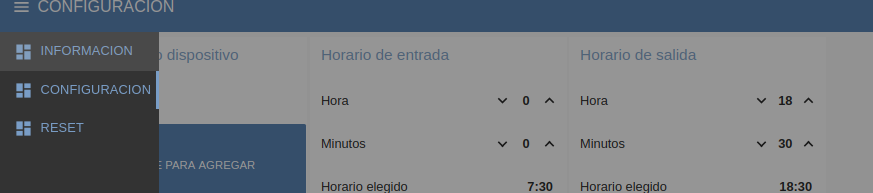
\includegraphics[width=0.8\textwidth]{./Figures/interfaz4.png}
	\caption{Solapa de información.}
	\label{fig:interfaz4}
\end{figure}

En la figura [\ref{fig:interfaz52}] se muestran los botones que provee la pagina web para el encedido y apagado de luz, también se ve el estado actual. Una vez presionado el botón {\textit{ON}} se puede ver en la figura [\ref{fig:interfaz51}] el envío del comando al nodo y la recepción del {\textit{ACK}}. Luego el sistema envía el comando {\textit{Get}} automáticamente para corroborar el cambio y actualizar el estado en la interfaz web.

\begin{figure}[h!]
	\centering
	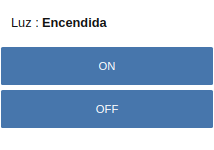
\includegraphics[width=0.3\textwidth]{./Figures/interfaz52.png}
	\caption{Interfaz web luego de presionar el botón {\textit{ON}}.}
	\label{fig:interfaz52}
\end{figure}

\begin{figure}[h!]
	\centering
	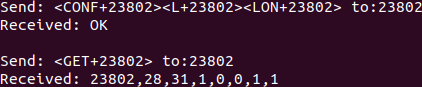
\includegraphics[width=0.6\textwidth]{./Figures/interfaz51.png}
	\caption{Envío y recepción de comandos después de presionar el botón {\textit{ON}}.}
	\label{fig:interfaz51}
\end{figure}

En las figuras [\ref{fig:interfaz62}] y [\ref{fig:interfaz61}] se puede ver el mismo mecanismo utilizado anteriormente en las figuras [\ref{fig:interfaz52}] y [\ref{fig:interfaz51}] pero en este caso se apaga la luz.

\begin{figure}[h!]
	\centering
	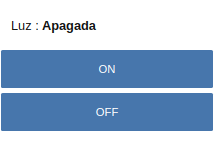
\includegraphics[width=0.3\textwidth]{./Figures/interfaz62.png}
	\caption{Interfaz web luego de presionar el botón {\textit{OFF}}.}
	\label{fig:interfaz62}
\end{figure}

\begin{figure}[h!]
	\centering
	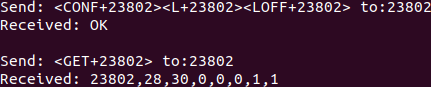
\includegraphics[width=0.6\textwidth]{./Figures/interfaz61.png}
	\caption{Envío y recepción de comandos después de presionar el botón {\textit{OFF}}.}
	\label{fig:interfaz61}
\end{figure}


\subsubsection{Pruebas de encendido y apagado del aire acondicionado}

De la misma manera que en la prueba anterior,se procedió a ensayar el encendido y apagado del aire acondicionado, para ésto se siguen los pasos:

\begin{enumerate}
\item Hacer click en la solapa {\textit{Información}}.
\item Elegir la marca del aire acondicionado.
\item Hacer click en {\textit{ON}}.
\item Hacer click en {\textit{OFF}}.
\end{enumerate}

En la figura [\ref{fig:interfaz71}] se muestra la apertura del menú que contiene las marcas de aires acondicionados y se selecciona una.
%
\begin{figure}[h!]
	\centering
	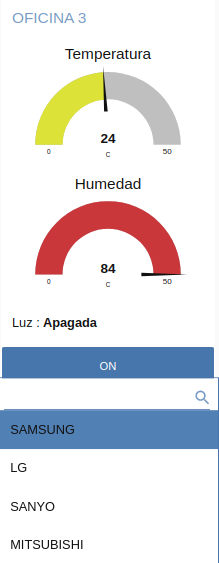
\includegraphics[width=0.2\textwidth]{./Figures/interfaz71.png}
	\caption{Selección de la marca del aire acondicionado en la interfaz de usuario.}
	\label{fig:interfaz71}
\end{figure}

Una vez seleccionada la marca, se muestra en la figura [\ref{fig:interfaz70}] el correspondiente envío del comando al nodo y la respuesta de éste.

\begin{figure}[h!]
	\centering
	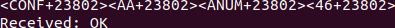
\includegraphics[width=0.6\textwidth]{./Figures/interfaz70.png}
	\caption{Envío y recepción de comandos por la terminal.}
	\label{fig:interfaz70}
\end{figure}

En la figura [\ref{fig:interfaz72}] se muestra el estado actual y los botones que provee la interfaz para el encendido y apagado del aire acondicionado.

\begin{figure}[h!]
	\centering
	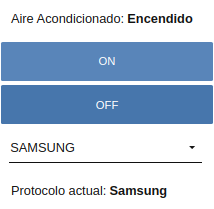
\includegraphics[width=0.3\textwidth]{./Figures/interfaz72.png}
	\caption{Interfaz web luego de presionar el botón {\textit{ON}}.}
	\label{fig:interfaz72}
\end{figure}

En la figura [\ref{fig:interfaz73}] se ve el envío del comando de encendido del aire acondicionado y la respuesta del nodo.

\begin{figure}[h!]
	\centering
	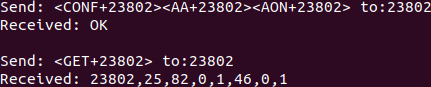
\includegraphics[width=0.6\textwidth]{./Figures/interfaz73.png}
	\caption{Envío y recepción de comandos por la terminal.}
	\label{fig:interfaz73}
\end{figure}

En las figuras [\ref{fig:interfaz81}] y [\ref{fig:interfaz82}] se puede ver el mismo mecanismo utilizado anteriormente en las figuras [\ref{fig:interfaz72}] y [\ref{fig:interfaz73}] pero en este caso se apaga el aire acondicionado.

\begin{figure}[ht!]
	\centering
	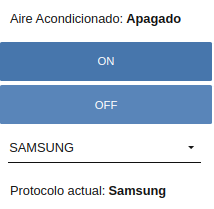
\includegraphics[width=0.3\textwidth]{./Figures/interfaz81.png}
	\caption{Interfaz web luego de presionar el botón {\textit{OFF}}.}
	\label{fig:interfaz81}
\end{figure}

\begin{figure}[ht!]
	\centering
	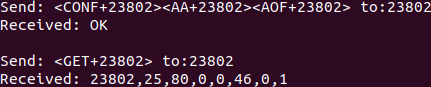
\includegraphics[width=0.6\textwidth]{./Figures/interfaz82.png}
	\caption{Envío y recepción de comandos por la terminal.}
	\label{fig:interfaz82}
\end{figure}


\subsubsection{Pruebas de sensor de temperatura y humedad}

En este ensayo se corrobora que los datos mostrados en la interfaz web acerca del sensor de temperatura y humedad se corresponden con los datos recibidos por el nodo.

En las figura [\ref{fig:interfaz90}] se pueden ver los datos recibidos por el nodo luego de que el sistema le mande un comando {\textit{Get}} al nodo, en las columnas 2 y 3 se puede ver el valor de temperatura y humedad respectivamente, y en la figura [\ref{fig:interfaz91}] se muestra la interfaz web y se corrobora el correcto funcionamiento de la interfaz mostrando los valores reales recibidos.

\begin{figure}[ht!]
	\centering
	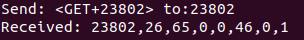
\includegraphics[width=0.5\textwidth]{./Figures/interfaz90.png}
	\caption{Recepción de datos, después del envío del comando {\textit{Get}} }
	\label{fig:interfaz90}
\end{figure}

\begin{figure}[ht!]
	\centering
	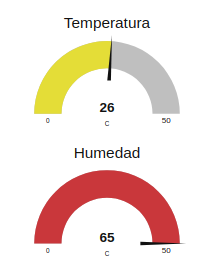
\includegraphics[width=0.3\textwidth]{./Figures/interfaz91.png}
	\caption{Interfaz web con los datos de temperatura y humedad}
	\label{fig:interfaz91}
\end{figure}

\subsubsection{Pruebas de detección de movimiento}

En esta sección se ensaya el uso del sensor de movimiento. Los pasos realizados fueron:

\begin{enumerate}
\item Hacer click en la solapa {\textit{Información}}.
\item Poner el sistema en modo Automático.
\item Activar la detección de movimiento.
\end{enumerate}

El sistema se pone en modo automático mediante el uso del botón {\textit{Modo}} que se encuentra en el nodo, pero también se lo puede hacer mediante la interfaz web.

En la figura [\ref{fig:interfaz10}] se puede ver que la interfaz web nos indica que el sistema se encuentra en modo automático y además provee los botones para activar y desactivar el sensor de movimiento.

\begin{figure}[h!]
	\centering
	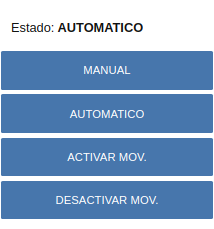
\includegraphics[width=0.3\textwidth]{./Figures/interfaz10.png}
	\caption{Interfaz web con el sistema en modo automático.}
	\label{fig:interfaz10}
\end{figure}

Se puede ver en la figura [\ref{fig:interfaz11}] que luego del paso 3, se activa el sensor de movimiento y al pasar un objeto por delante, el sistema lo detecta y activa una ventana de emergencia en la interfaz web.

\begin{figure}[ht!]
	\centering
	\includegraphics[width=0.8\textwidth]{./Figures/interfaz11.png}
	\caption{Interfaz web con ventana pop-up indicando una alerta de movimiento en el sector 3}
	\label{fig:interfaz11}
\end{figure}


\subsubsection{Resultados}

\begin{itemize}
\item Se comprobó que la interfaz web funciona correctamente.
\item Los comandos son enviados y recibidos correctamente.
\item La sincronización de hilos en la aplicación funciona como es esperado.
\end{itemize}
 
% Chapter Template

\chapter{Conclusiones} % Main chapter title

\label{Chapter5} % Change X to a consecutive number; for referencing this chapter elsewhere, use \ref{ChapterX}

En este capítulo se realiza un resumen sobre los conocimientos aplicados, el trabajo realizado hasta el momento y problemas que surgieron durante el desarrollo.

%----------------------------------------------------------------------------------------

%----------------------------------------------------------------------------------------
%	SECTION 1
%----------------------------------------------------------------------------------------

\section{Trabajo realizado }

En la presente memoria se documentó la implementación de un prototipo de domótica para edificios públicos. Particularmente se implemento el monitoreo de temperatura y humedad, el control de encendido y apagado de luces y aires acondicionados para diferentes marcas y la detección de movimiento en el área.

Se desarrolló e implementó satisfactoriamente una red de nodos que responden a una central y que proveen una estructura de servicios propia y local sin necesidad de una red Wi-Fi. La implementación permite, no solo generar eficiencia energética en edificios públicos de gran tamaño, sino también la detección de movimiento en las oficinas o áreas donde se encuentre un nodo. Ésto es importante para generar una alarma preventiva. También presenta una interfaz de visualización de fácil uso para el usuario.

Se hicieron modificaciones de los requisitos a lo largo del proyecto debido al planteo del cliente. Los requisitos no fueron cumplidos en su totalidad, quedando para una segunda etapa las tareas de diseño de un hardware mas pequeño como así también las pruebas en planta.

Surgieron nuevos riesgos que no estaban considerados al plantear el proyecto y que no pudieron ser mitigados con satisfacción. No obstante, se concluye que la mayoría de los objetivos planteados al comienzo del trabajo fueron alcanzados satisfactoriamente y se han obtenido conocimientos valiosos para la formación del autor.



%\begin{itemize}
%\item ¿Cuál es el grado de cumplimiento de los requerimientos?
%\item ¿Cuán fielmente se puedo seguir la planificación original (cronograma incluido)?
%\item ¿Se manifestó algunos de los riesgos identificados en la planificación? ¿Fue efectivo el plan de mitigación? ¿Se debió aplicar alguna otra acción no contemplada previamente?
%\item Si se debieron hacer modificaciones a lo planificado ¿Cuáles fueron las causas y los efectos?
%\item ¿Qué técnicas resultaron útiles para el desarrollo del proyecto y cuáles no tanto?
%\end{itemize}


%----------------------------------------------------------------------------------------
%	SECTION 2
%----------------------------------------------------------------------------------------
\section{Conocimientos aplicados }

Durante el desarrollo del este trabajo se aplicaron conocimientos adquiridos a lo largo del año en la Especialización de Sistemas Embebidos. Todas las asignaturas cursadas aportaron conocimientos necesarios para que el trabajo finalmente se encuentre funcionando. Sin embargo, se resaltan a continuación aquellas materias de mayor relevancia para este trabajo.

\begin{itemize}
\item Gestión de Proyectos: la elaboración de un plan de proyecto para organizar el trabajo final, facilitó la realización del mismo.
\item Ingeniería de Software en Sistemas Embebidos: la creación de un documento de especificaciones de requerimientos permitió ordenar y documentar las necesidades del cliente además de enseñar el uso de sistemas de control de versiones.
\item Protocolos de Comunicación: resulto de utilidad para la creación del driver de uno de los componentes.
\item Sistemas Operativos de Propósito General: se aplicaron conceptos de uso de hilos y procesos, como también de sincronización entre procesos y uso de variables compartidas.
\item Desarrollo de Aplicaciones en Sistemas Operativos: se aplicaron conocimientos del lenguaje de programación Python, uso de ficheros y la programación orientada a objeto.
\item Diseño de Circuitos Impresos: aportó al uso de la herramienta libre KiCad.
\end{itemize}


%----------------------------------------------------------------------------------------
%	SECTION 3
%----------------------------------------------------------------------------------------
\section{Trabajo futuro }

Resulta imprescindible identificar el trabajo futuro, para dar continuidad al esfuerzo realizado hasta el momento y poder realizar un producto comercialmente atractivo. A continuación se listan las líneas de trabajo mas importantes:

\begin{itemize}
\item Diseñar un prototipo de hardware más pequeño para su uso dentro de cajas de electricidad convencionales.
\item Modificar la interfaz web para agregar nodos de forma automática.
\item Separar los leds infrarrojos del nodo para poder situarlos mas cerca del aire acondicionado.
\item Agregar la posibilidad de actualizar el firmware del gateway de forma remota.
\end{itemize}



 

%----------------------------------------------------------------------------------------
%	CONTENIDO DE LA MEMORIA  - APÉNDICES
%----------------------------------------------------------------------------------------

\appendix % indicativo para indicarle a LaTeX los siguientes "capítulos" son apéndices

% Incluir los apéndices de la memoria como archivos separadas desde la carpeta Appendices
% Descomentar las líneas a medida que se escriben los apéndices

%\include{Appendices/AppendixA}
%\include{Appendices/AppendixB}
%\include{Appendices/AppendixC}

%----------------------------------------------------------------------------------------
%	BIBLIOGRAPHY
%----------------------------------------------------------------------------------------


\Urlmuskip=0mu plus 1mu\relax
\raggedright
\printbibliography[heading=bibintoc]

%----------------------------------------------------------------------------------------

\end{document}  
